% ==========================================================================
%  Chapter 1: A Primer on Linear Algebra
%  Publication-Quality Expanded Version
% ==========================================================================
\chapter{A Primer on Linear Algebra}
\label{ch:linear_algebra}

\epigraph{%
  A useful model connects a mathematical description to measurements, forces and motion.
}{}

\begin{laymansbox}{Context and Use Case: Linear Algebra for Motion}{ch1_context_box}
\textbf{The Math You Will See:} We will cover Vectors ($\mathbf{v}$), Matrices ($\mathbf{M}$), Vector Spaces and their axioms, Linear Independence and Basis, Eigenvalues/Eigenvectors ($\lambda, \mathbf{v}$), the Singular Value Decomposition (SVD), Quadratic Forms ($\mathbf{x}^T \mathbf{M} \mathbf{x}$), Positive Definiteness, and Dyads/Dyadics (the tensor products that underpin inertia, stress, and stiffness).

\textbf{Why We Need It:} Joint velocities, task velocities, forces and measured signals have multiple interacting components. Linear maps describe how those components relate at a specified state; matrix decompositions reveal directions, sensitivity and numerical structure. Predicting a collision or a golf shot additionally requires the dynamics, initial condition, inputs, constraints and contact event. Eigenvalues of one matrix do not answer all of those questions.

\textbf{All Variables Defined:} Check the \textbf{Nomenclature} at the start of the book for standard vector and matrix conventions.
\end{laymansbox}

% ------------------------------------------------------------------
\section{Historical Context}
\label{sec:la_history}
% ------------------------------------------------------------------

Linear algebra connects the problem of solving simultaneous equations with the geometric study of linear transformations. Its importance in mechanics comes from reusing the same structure for different tasks: resolving velocities, assembling inertias, fitting measurements and propagating local perturbations.

Kalman's 1960 paper \emph{A New Approach to Linear Filtering and Prediction Problems} used state-transition methods to derive a recursive linear estimation scheme and its error-covariance equations~\cite{Kalman1960}. It was a major contribution to estimation, not the first invention of state representation or a claim that every physical system is linear. Controllability and observability make the role of matrix rank precise for declared dynamical models.

Modern simulation and optimization combine kinematic maps, linear solves and nonlinear updates. Solving a linear system within a nonlinear simulation does not make the entire simulated motion linear. The algebra keeps those uses distinct.

% ------------------------------------------------------------------
\section{Vectors, Matrices, and Vector Spaces}
\label{sec:vectors_matrices}
% ------------------------------------------------------------------

Before mapping physics, we must understand the fundamental data structures of control theory: vectors and matrices. More importantly, we must understand the abstract \emph{space} in which these objects live, because the space and its metric determine which operations and comparisons are meaningful. Readers seeking a comprehensive undergraduate treatment of these ideas will find Strang's textbook~\cite{strang2019} an excellent companion to this chapter.

\begin{figure}[htb]
\centering
\begin{tikzpicture}[scale=1.0]
  % Draw 3D coordinate system
  \draw[->] (0,0,0) -- (3,0,0) node[anchor=west] {$x_1$};
  \draw[->] (0,0,0) -- (0,3,0) node[anchor=south] {$x_2$};
  \draw[->] (0,0,0) -- (0,0,3) node[anchor=east] {$x_3$};

  % Draw a vector
  \draw[->,thick,blue] (0,0,0) -- (2,1.5,1.5) node[anchor=west] {$\mathbf{v}$};

  % Draw projection onto x1-x2 plane
  \draw[dashed,gray] (2,1.5,1.5) -- (2,1.5,0);
  \draw[dashed,gray] (2,1.5,0) -- (0,0,0);

  % Draw a transformation (linear transformation visualization)
  \draw[thick,red,->] (5,1,0.75) -- (7,2.25,1.5) node[anchor=west] {$\mathbf{M}\mathbf{v}$};
  \node at (6,0,0) {Linear Transformation};
\end{tikzpicture}
\caption{Vector in $\Reals^3$ and its transformation under a linear map $T(\mathbf{v}) = \mathbf{M}\mathbf{v}$.}
\label{fig:vector_transformation}
\end{figure}

\subsection{Vectors}

An element of a vector space is a \textbf{vector}\index{Vector}; after choosing a finite basis, its coordinates form an ordered array of numbers. It can represent a position in space, a velocity profile, a list of sensor readings, or the activation levels of every muscle in a golfer's forearm. In physics, vectors implicitly assume a coordinate frame (e.g., $X, Y, Z$). A generic column vector in $n$-dimensional space is denoted:
\begin{equation}
   \mathbf{v} = \begin{bmatrix} v_1 \\ v_2 \\ \vdots \\ v_n \end{bmatrix} \in \Reals^n
\end{equation}

It is crucial to distinguish two perspectives on what a vector ``is.'' The \emph{algebraic} perspective treats a vector as a column of numbers. The \emph{geometric} perspective treats a vector as a directed arrow in space, possessing both magnitude and direction. Both perspectives are useful when the basis and metric are stated. A position is a point in an affine space; displacement and velocity are vectors. Muscle activations can be stored in an array, but their physically admissible bounded, nonnegative set is not itself a real vector space. When we write $\mathbf{v} \in \Reals^3$, we mean both the triple of numbers $(v_1, v_2, v_3)$ and the arrow pointing from the origin to the point $(v_1, v_2, v_3)$ in three-dimensional Euclidean space.

\subsection{Matrices}

A \textbf{matrix}\index{Matrix} $\mathbf{M}$ is a rectangular grid of numbers arranged in rows and columns. If a vector represents a point or a direction, a matrix acts as a set of instructions on how to \emph{transform} that point---stretching it, rotating it, projecting it, or mapping it into an entirely different dimensional space. An $n \times m$ matrix maps vectors from $\Reals^m$ to $\Reals^n$:
\begin{equation}
   \mathbf{M} = \begin{bmatrix} m_{11} & m_{12} & \cdots & m_{1m} \\ m_{21} & m_{22} & \cdots & m_{2m} \\ \vdots & \vdots & \ddots & \vdots \\ m_{n1} & m_{n2} & \cdots & m_{nm} \end{bmatrix} \in \Reals^{n \times m}
\end{equation}

When we multiply a matrix by a vector ($\mathbf{M}\mathbf{v}$), the result is a \emph{linear combination of the columns of} $\mathbf{M}$, using the elements of $\mathbf{v}$ as weights. Specifically, if $\mathbf{m}_1, \mathbf{m}_2, \ldots, \mathbf{m}_m$ denote the columns of $\mathbf{M}$, then:
\begin{equation}
\label{eq:matvec_colview}
   \mathbf{M}\mathbf{v} = v_1 \mathbf{m}_1 + v_2 \mathbf{m}_2 + \cdots + v_m \mathbf{m}_m
\end{equation}
This ``column view'' of matrix-vector multiplication is one of the most important conceptual tools in linear algebra. It means that the \emph{range} (or image) of a matrix---the set of all possible outputs $\mathbf{M}\mathbf{v}$ as $\mathbf{v}$ varies over all of $\Reals^m$---is precisely the \emph{span} of the columns of $\mathbf{M}$. Throughout this book, when we rotate a robot arm, we are physically applying a matrix to the vectors extending along its links.

\subsection{The Axioms of a Vector Space}
\label{subsec:vector_space_axioms}

We have described vectors informally as ``arrays of numbers.'' But the true power of linear algebra lies in the abstract concept of a \textbf{vector space}\index{Vector Space}, which captures the essential algebraic properties that make vectors useful---regardless of whether the ``vectors'' are columns of numbers, functions, or even infinite-dimensional signals.

\begin{definition}{Vector Space}{vector_space}
A \emph{vector space} $V$ over the real numbers $\Reals$ is a set of objects (called vectors) together with two operations---\textbf{addition} ($\mathbf{u} + \mathbf{v}$) and \textbf{scalar multiplication} ($\alpha \mathbf{v}$, where $\alpha \in \Reals$)---satisfying the following eight axioms for all $\mathbf{u}, \mathbf{v}, \mathbf{w} \in V$ and all $\alpha, \beta \in \Reals$:

\begin{enumerate}[label=(\roman*)]
    \item \textbf{Closure under addition:} $\mathbf{u} + \mathbf{v} \in V$.
    \item \textbf{Commutativity:} $\mathbf{u} + \mathbf{v} = \mathbf{v} + \mathbf{u}$.
    \item \textbf{Associativity of addition:} $(\mathbf{u} + \mathbf{v}) + \mathbf{w} = \mathbf{u} + (\mathbf{v} + \mathbf{w})$.
    \item \textbf{Existence of a zero vector:} There exists $\mathbf{0} \in V$ such that $\mathbf{v} + \mathbf{0} = \mathbf{v}$.
    \item \textbf{Existence of additive inverses:} For each $\mathbf{v} \in V$, there exists $-\mathbf{v} \in V$ such that $\mathbf{v} + (-\mathbf{v}) = \mathbf{0}$.
    \item \textbf{Closure under scalar multiplication:} $\alpha \mathbf{v} \in V$.
    \item \textbf{Distributivity:} $\alpha(\mathbf{u} + \mathbf{v}) = \alpha \mathbf{u} + \alpha \mathbf{v}$ \; and \; $(\alpha + \beta)\mathbf{v} = \alpha \mathbf{v} + \beta \mathbf{v}$.
    \item \textbf{Compatibility:} $\alpha(\beta \mathbf{v}) = (\alpha\beta)\mathbf{v}$, \; and \; $1 \cdot \mathbf{v} = \mathbf{v}$.
\end{enumerate}
\end{definition}

\begin{laymansbox}{Why Do We Care About Abstract Axioms?}{axiom_motivation}
You might wonder: why bother with these formal rules? Because the same mathematical structures appear over and over in radically different contexts. The set $\Reals^n$ of column vectors satisfies these axioms---but so does the set of all continuous functions $f: [0, T] \to \Reals$ (where ``addition'' means adding functions pointwise). In optimal control, the ``vectors'' we optimize over are often entire \emph{trajectories}, which are functions of time. By proving a theorem about abstract vector spaces, we prove it simultaneously for column vectors, for functions, and for trajectories. The axioms are the price of generality. The ambient function space may be a vector space, but trajectories satisfying nonlinear dynamics, unilateral contact or bounded actuation generally form a constrained subset that is not closed under addition and scaling.
\end{laymansbox}

\begin{example}{Verifying \texorpdfstring{$\Reals^n$}{Rn} is a Vector Space}{rn_vector_space}
Let us verify that $\Reals^n$ with standard component-wise addition and scalar multiplication satisfies the axioms.

Given $\mathbf{u} = (u_1, \ldots, u_n)$ and $\mathbf{v} = (v_1, \ldots, v_n)$ in $\Reals^n$, and $\alpha \in \Reals$:
\begin{itemize}
    \item \emph{Closure under addition:} $\mathbf{u} + \mathbf{v} = (u_1 + v_1, \ldots, u_n + v_n)$. Since each $u_i + v_i \in \Reals$, the sum is in $\Reals^n$. \checkmark
    \item \emph{Zero vector:} $\mathbf{0} = (0, 0, \ldots, 0)$. Clearly $\mathbf{v} + \mathbf{0} = \mathbf{v}$. \checkmark
    \item \emph{Additive inverse:} $-\mathbf{v} = (-v_1, \ldots, -v_n)$. Then $\mathbf{v} + (-\mathbf{v}) = \mathbf{0}$. \checkmark
    \item \emph{Closure under scalar multiplication:} $\alpha \mathbf{v} = (\alpha v_1, \ldots, \alpha v_n) \in \Reals^n$. \checkmark
\end{itemize}
The remaining axioms (commutativity, associativity, distributivity, compatibility) follow immediately from the corresponding properties of real number arithmetic. Therefore $\Reals^n$ is a vector space. $\square$
\end{example}

\subsection{Linear Independence and Span}
\label{subsec:linear_independence}

\begin{definition}{Linear Independence\index{Linear Independence}}{linear_independence}
A set of vectors $\{\mathbf{v}_1, \mathbf{v}_2, \ldots, \mathbf{v}_k\}$ in a vector space $V$ is called \emph{linearly independent} if the only solution to the equation
\begin{equation}
    \alpha_1 \mathbf{v}_1 + \alpha_2 \mathbf{v}_2 + \cdots + \alpha_k \mathbf{v}_k = \mathbf{0}
\end{equation}
is the trivial solution $\alpha_1 = \alpha_2 = \cdots = \alpha_k = 0$. If a nontrivial solution exists (i.e., at least one $\alpha_i \neq 0$), the vectors are \emph{linearly dependent}.
\end{definition}

Intuitively, a set of vectors is linearly independent if none of them can be ``built'' from the others. In $\Reals^2$, two nonzero vectors are independent exactly when neither is a scalar multiple of the other. In $\Reals^3$, three vectors are independent exactly when they do not lie in one plane through the origin.

\begin{example}{Linear Independence in \texorpdfstring{$\Reals^3$}{R3}}{lin_indep_R3}
Consider the vectors:
\begin{equation}
    \mathbf{v}_1 = \begin{bmatrix} 1 \\ 0 \\ 0 \end{bmatrix}, \quad
    \mathbf{v}_2 = \begin{bmatrix} 0 \\ 1 \\ 0 \end{bmatrix}, \quad
    \mathbf{v}_3 = \begin{bmatrix} 1 \\ 1 \\ 0 \end{bmatrix}
\end{equation}

Are these linearly independent? We solve $\alpha_1 \mathbf{v}_1 + \alpha_2 \mathbf{v}_2 + \alpha_3 \mathbf{v}_3 = \mathbf{0}$:
\begin{align}
    \alpha_1 + \alpha_3 &= 0 \\
    \alpha_2 + \alpha_3 &= 0 \\
    0 &= 0
\end{align}

The third equation provides no constraint. Setting $\alpha_3 = 1$ yields $\alpha_1 = -1$, $\alpha_2 = -1$. A nontrivial solution exists: $-\mathbf{v}_1 - \mathbf{v}_2 + \mathbf{v}_3 = \mathbf{0}$, confirming that $\mathbf{v}_3 = \mathbf{v}_1 + \mathbf{v}_2$. The vectors are linearly \emph{dependent}. Geometrically, all three vectors lie in the $xy$-plane, and the third is the diagonal of the rectangle formed by the first two.
\end{example}

\subsection{Basis and Dimension}
\label{subsec:basis_dimension}

\begin{definition}{Basis\index{Basis}}{basis}
A finite \emph{basis} for a finite-dimensional vector space $V$ is a set of vectors $\mathcal{B} = \{\mathbf{b}_1, \ldots, \mathbf{b}_n\}$ that is both linearly independent and spans $V$ (i.e., every vector in $V$ can be written as a linear combination of the basis vectors). The number $n$ of vectors in any basis is called the \emph{dimension}\index{Dimension} of $V$, written $\dim(V) = n$.
\end{definition}

A fundamental theorem of linear algebra states that \emph{every basis for a given vector space has exactly the same number of elements}. This is why ``dimension'' is well-defined---it is an intrinsic property of the space, not of any particular choice of basis.

The standard basis for $\Reals^n$ consists of the unit coordinate vectors $\mathbf{e}_1 = (1, 0, \ldots, 0)^T$, $\mathbf{e}_2 = (0, 1, 0, \ldots, 0)^T$, through $\mathbf{e}_n = (0, \ldots, 0, 1)^T$. Any vector $\mathbf{v} = (v_1, \ldots, v_n)^T$ can be written uniquely as $\mathbf{v} = v_1 \mathbf{e}_1 + \cdots + v_n \mathbf{e}_n$. The numbers $v_1, \ldots, v_n$ are the \emph{coordinates} of $\mathbf{v}$ with respect to this basis.

\begin{laymansbox}{Why Basis Matters for Robotics}{basis_robotics}
Joint angles are coordinates on a configuration space, not basis vectors. A task map $\mathbf y=h(\mathbf q)$ is generally nonlinear and can change dimension. Its Jacobian $J(\mathbf q)=Dh(\mathbf q)$ maps an instantaneous joint velocity to a task velocity, $\dot{\mathbf y}=J\dot{\mathbf q}$. This is a linear map between tangent spaces at a specified configuration, and may have a nontrivial kernel. A change of basis within one finite-dimensional vector space is instead square and invertible. A seven-joint-to-three-position Jacobian cannot be a change of basis.

\end{laymansbox}

\subsection{Linear Transformations}
\label{subsec:linear_transformations}

\begin{definition}{Linear Transformation\index{Linear Transformation}}{linear_transformation}
A function $T: V \to W$ between two vector spaces is called a \emph{linear transformation} (or \emph{linear map}) if it preserves vector addition and scalar multiplication:
\begin{enumerate}[label=(\roman*)]
    \item $T(\mathbf{u} + \mathbf{v}) = T(\mathbf{u}) + T(\mathbf{v})$ for all $\mathbf{u}, \mathbf{v} \in V$.
    \item $T(\alpha \mathbf{v}) = \alpha \, T(\mathbf{v})$ for all $\alpha \in \Reals$ and $\mathbf{v} \in V$.
\end{enumerate}
\end{definition}

The fundamental connection between linear transformations and matrices is this: \emph{every linear transformation between finite-dimensional vector spaces can be represented by a matrix, and every matrix represents a linear transformation.} Specifically, if $T: \Reals^m \to \Reals^n$ is linear, then there exists a unique $n \times m$ matrix $\mathbf{M}$ such that $T(\mathbf{v}) = \mathbf{M}\mathbf{v}$ for all $\mathbf{v} \in \Reals^m$. The columns of $\mathbf{M}$ are simply $T(\mathbf{e}_1), T(\mathbf{e}_2), \ldots, T(\mathbf{e}_m)$---the images of the standard basis vectors.

\begin{theorem}{Matrix Multiplication is Linear}{matrix_is_linear}
Let $\mathbf{M} \in \Reals^{n \times m}$. Then the function $T(\mathbf{v}) = \mathbf{M}\mathbf{v}$ is a linear transformation from $\Reals^m$ to $\Reals^n$.
\end{theorem}

\begin{proof}
Let $\mathbf{u}, \mathbf{v} \in \Reals^m$ and $\alpha \in \Reals$. By the distributive property of matrix multiplication:
\begin{equation}
    T(\mathbf{u} + \mathbf{v}) = \mathbf{M}(\mathbf{u} + \mathbf{v}) = \mathbf{M}\mathbf{u} + \mathbf{M}\mathbf{v} = T(\mathbf{u}) + T(\mathbf{v})
\end{equation}
and by the compatibility of matrix multiplication with scalar multiplication:
\begin{equation}
    T(\alpha \mathbf{v}) = \mathbf{M}(\alpha \mathbf{v}) = \alpha (\mathbf{M}\mathbf{v}) = \alpha \, T(\mathbf{v})
\end{equation}
Both conditions of linearity are satisfied.
\end{proof}

\subsection{Rank, Null Space, and the Rank-Nullity Theorem}
\label{subsec:rank_nullity}

Not all linear transformations preserve full information about the input. Some transformations ``collapse'' certain directions to zero.

\begin{definition}{Rank\index{Rank}}{rank}
The \emph{rank} of a matrix $\mathbf{M}$, denoted $\text{rank}(\mathbf{M})$, is the number of linearly independent columns (equivalently, the number of linearly independent rows) of $\mathbf{M}$. It equals the dimension of the column space (the range of the corresponding linear transformation).
\end{definition}

If a $3 \times 3$ matrix has rank 2, it collapses full 3D space into a 2D plane. In robotics, the rank of the Jacobian matrix $\mathbf{J}(\mathbf{q})$ tells you how many independent directions the end-effector can instantaneously move in. If the rank drops below its maximum value, the robot is at a \emph{singularity}\index{Singularity}---some previously available instantaneous task velocities are no longer in its image. This statement concerns the chosen task and admissible joint velocities; it does not by itself prove finite-time unreachability or loss of dynamical controllability.

\begin{definition}{Null Space (Kernel)\index{Null Space}}{null_space}
The \emph{null space} (or \emph{kernel}) of a matrix $\mathbf{M}$, denoted $\mathcal{N}(\mathbf{M})$, is the set of all vectors that the matrix maps to zero:
\begin{equation}
    \mathcal{N}(\mathbf{M}) = \{ \mathbf{x} \in \Reals^m \mid \mathbf{M}\mathbf{x} = \mathbf{0} \}
\end{equation}
\end{definition}

For a redundant arm, $\ker J(\mathbf q)$ contains instantaneous joint velocities with zero velocity in the chosen hand task. A finite self-motion must keep satisfying the evolving constraint $J(\mathbf q(t))\dot{\mathbf q}(t)=0$; a straight step along the initial kernel need not do so. At regular configurations the constant-rank theorem describes the local task-level set. At a singular configuration, even an instantaneous kernel direction need not integrate into a finite constant-task motion.

\begin{definition}{The Determinant\index{Determinant} (Volumetric Interpretation)}{determinant}
For a square matrix $\mathbf{M} \in \Reals^{n \times n}$, the \emph{determinant} $\det(\mathbf{M})$ is a scalar whose absolute value measures the factor by which $\mathbf{M}$ scales $n$-dimensional volume. Imagine a unit hypercube $[0,1]^n$. Applying $\mathbf{M}$ to every point in that cube warps it into a parallelepiped whose signed volume equals $\det(\mathbf{M})$.
\end{definition}

\begin{itemize}
    \item If $\det(\mathbf{M}) = 1$, volume is perfectly preserved (like a pure rotation in space).
    \item If $\det(\mathbf{M}) = 0$, volume is crushed completely flat---the matrix is \emph{singular} and loses rank. The transformation is not invertible.
    \item If $\det(\mathbf{M}) < 0$, orientation is reversed and volume is multiplied by $|\det(\mathbf M)|$. For example, $\operatorname{diag}(-2,3)$ reverses orientation and multiplies area by six; only absolute determinant one preserves volume.
\end{itemize}

Now we arrive at one of the most important structural results in linear algebra:

\begin{theorem}{Rank-Nullity Theorem\index{Rank-Nullity Theorem}}{rank_nullity}
For any $n \times m$ matrix $\mathbf{M}$:
\begin{equation}
    \underbrace{\text{rank}(\mathbf{M})}_{\text{dimension of range}} + \underbrace{\dim\bigl(\mathcal{N}(\mathbf{M})\bigr)}_{\text{dimension of null space}} = m \quad (\text{number of columns})
\end{equation}
\end{theorem}

\begin{proof}
Let $r = \text{rank}(\mathbf{M})$ and let $\{\mathbf{n}_1, \ldots, \mathbf{n}_k\}$ be a basis for $\mathcal{N}(\mathbf{M})$, where $k = \dim(\mathcal{N}(\mathbf{M}))$. Extend this to a basis $\{\mathbf{n}_1, \ldots, \mathbf{n}_k, \mathbf{w}_1, \ldots, \mathbf{w}_{m-k}\}$ for all of $\Reals^m$ (this extension is always possible by a standard result in linear algebra).

We claim that $\{\mathbf{M}\mathbf{w}_1, \ldots, \mathbf{M}\mathbf{w}_{m-k}\}$ is a basis for the column space of $\mathbf{M}$, which would establish $r = m - k$, i.e., $r + k = m$.

\emph{Spanning:} Any $\mathbf{y}$ in the range of $\mathbf{M}$ can be written as $\mathbf{y} = \mathbf{M}\mathbf{v}$ for some $\mathbf{v} \in \Reals^m$. Expanding $\mathbf{v}$ in our basis: $\mathbf{v} = \sum_{i=1}^k \alpha_i \mathbf{n}_i + \sum_{j=1}^{m-k} \beta_j \mathbf{w}_j$. Since $\mathbf{M}\mathbf{n}_i = \mathbf{0}$, we get $\mathbf{y} = \sum_{j=1}^{m-k} \beta_j \mathbf{M}\mathbf{w}_j$. So the $\mathbf{M}\mathbf{w}_j$ span the range.

\emph{Independence:} Suppose
\[
\sum_{j=1}^{m-k}\beta_j\mathbf M\mathbf w_j=0.
\]
Then $M(\sum_j\beta_j\mathbf w_j)=0$, so the vector $\sum_j\beta_j\mathbf w_j$ belongs to the kernel. It therefore equals $\sum_{i=1}^k\gamma_i\mathbf n_i$ for some scalars $\gamma_i$. The combined list of kernel vectors and extension vectors is a basis for $\Reals^m$, so it is independent. All $\beta_j$ and $\gamma_i$ must be zero.

Thus $r = m - k$, establishing $\text{rank}(\mathbf{M}) + \dim(\mathcal{N}(\mathbf{M})) = m$.
\end{proof}

\begin{laymansbox}{The Physical Meaning of Rank-Nullity}{rank_nullity_physical}
For a robot with $m$ independent joint-velocity coordinates and an $n$-dimensional task:
\begin{itemize}
    \item The \textbf{rank} of the Jacobian tells you the dimension of the instantaneous task-velocity image when all declared joint velocities are admissible.
    \item The \textbf{nullity} (dimension of the null space) tells you how many ``extra'' internal motions remain after the task is specified.
\end{itemize}
If a 7-DOF arm ($m = 7$) controls a hand in 3D position space ($n = 3$), and the Jacobian has rank 3, then the nullity is $7 - 3 = 4$. The robot has 4 degrees of internal freedom to reposition its elbow, shoulder, and wrist with zero instantaneous hand-position velocity. This does not fix hand orientation or guarantee a finite self-motion without updating the Jacobian.
\end{laymansbox}

% ------------------------------------------------------------------
\section{The Dot Product, Cross Product, and Inner Product Spaces}
\label{sec:dot_cross}
% ------------------------------------------------------------------

Two fundamental operations exist for combining vectors. Understanding them geometrically is essential for everything from computing kinetic energy to defining stability metrics.

\subsection{The Dot Product (Inner Product)}
\label{subsec:dot_product}

The dot product (or inner product) takes two vectors and returns a scalar. It measures how much two vectors ``align'' with each other.

\begin{definition}{Dot Product\index{Dot Product}}{dot_product}
In an orthonormal Euclidean basis, the \emph{dot product} of vectors $\mathbf{a}, \mathbf{b} \in \Reals^n$ is:
\begin{equation}
   \mathbf{a} \cdot \mathbf{b} = \mathbf{a}^T \mathbf{b} = \sum_{i=1}^n a_i b_i
\end{equation}
In $\Reals^3$, this expands to $a_x b_x + a_y b_y + a_z b_z$.
\end{definition}

The geometric interpretation connects the algebraic formula to angles:
\begin{equation}
\label{eq:dot_product_angle}
   \mathbf{a} \cdot \mathbf{b} = \norm{\mathbf{a}}\norm{\mathbf{b}}\cos(\theta)
\end{equation}
where $\theta$ is the angle between $\mathbf{a}$ and $\mathbf{b}$, and $\norm{\mathbf{a}} = \sqrt{\mathbf{a} \cdot \mathbf{a}}$ is the Euclidean norm (length) of $\mathbf{a}$.

\begin{proof}[Derivation of Equation~\eqref{eq:dot_product_angle}]
Consider two vectors $\mathbf{a}$ and $\mathbf{b}$ with an angle $\theta$ between them. The vector $\mathbf{a} - \mathbf{b}$ forms the third side of a triangle. By the law of cosines:
\begin{equation}
    \norm{\mathbf{a} - \mathbf{b}}^2 = \norm{\mathbf{a}}^2 + \norm{\mathbf{b}}^2 - 2\norm{\mathbf{a}}\norm{\mathbf{b}}\cos\theta
\end{equation}
Expanding the left side using the definition of the norm:
\begin{align}
    \norm{\mathbf{a} - \mathbf{b}}^2 &= (\mathbf{a} - \mathbf{b})^T(\mathbf{a} - \mathbf{b}) \\
    &= \mathbf{a}^T\mathbf{a} - 2\mathbf{a}^T\mathbf{b} + \mathbf{b}^T\mathbf{b} \\
    &= \norm{\mathbf{a}}^2 - 2\,\mathbf{a}^T\mathbf{b} + \norm{\mathbf{b}}^2
\end{align}
Equating the two expressions:
\begin{equation}
    \norm{\mathbf{a}}^2 - 2\,\mathbf{a}^T\mathbf{b} + \norm{\mathbf{b}}^2 = \norm{\mathbf{a}}^2 + \norm{\mathbf{b}}^2 - 2\norm{\mathbf{a}}\norm{\mathbf{b}}\cos\theta
\end{equation}
Canceling $\norm{\mathbf{a}}^2 + \norm{\mathbf{b}}^2$ from both sides and dividing by $-2$:
\begin{equation}
    \mathbf{a}^T\mathbf{b} = \norm{\mathbf{a}}\norm{\mathbf{b}}\cos\theta
\end{equation}
\end{proof}

Key consequences of the dot product formula:
\begin{itemize}
    \item If $\theta = 0$ (parallel vectors): $\mathbf{a} \cdot \mathbf{b} = \norm{\mathbf{a}}\norm{\mathbf{b}}$ (maximum positive value).
    \item If $\theta = 90^\circ$ (perpendicular vectors): $\mathbf{a} \cdot \mathbf{b} = 0$. This is the fundamental test for \textbf{orthogonality}\index{Orthogonality}.
    \item If $\theta = 180^\circ$ (antiparallel vectors): $\mathbf{a} \cdot \mathbf{b} = -\norm{\mathbf{a}}\norm{\mathbf{b}}$ (maximum negative value).
\end{itemize}

In mechanics, $T=\frac12\dot{\mathbf q}^TM(\mathbf q)\dot{\mathbf q}$ is a kinetic-energy quadratic form. An optimal-control running cost may be $\ell=\mathbf x^TQ\mathbf x+\mathbf u^TR\mathbf u$; a trajectory cost integrates it and may add a terminal cost. Generalized-force projection $\tau_i=\mathcal F^T\mathcal S_i$ is a dual pairing of a wrench and a joint-motion direction, with consistent frame, reference point and component order. These expressions have different units and meanings; none is automatically a Euclidean angle between like physical quantities.

\subsubsection{Orthogonal Projection}

A common operation is projecting one vector onto another. For $\mathbf a\ne0$, the \textbf{scalar projection} is $\mathbf a^T\mathbf b/\|\mathbf a\|$. The \textbf{vector projection} is:
\begin{equation}
    \text{proj}_{\mathbf{a}} \mathbf{b} = \frac{\mathbf{a} \cdot \mathbf{b}}{\mathbf{a} \cdot \mathbf{a}} \, \mathbf{a} = \frac{\mathbf{a}^T \mathbf{b}}{\norm{\mathbf{a}}^2} \, \mathbf{a}
\end{equation}
The residual $\mathbf{b} - \text{proj}_{\mathbf{a}} \mathbf{b}$ is orthogonal to $\mathbf{a}$. This decomposition---splitting a vector into a component along a direction and a component perpendicular to it---is the geometric core of the Gram-Schmidt process and underlies the QR decomposition used in numerical linear algebra.

\subsection{The Cross Product and the Skew-Symmetric Matrix}
\label{subsec:cross_product}

The standard cross product used here is defined in oriented three-dimensional Euclidean space. Its result is orthogonal to both inputs. Parallel inputs, or a zero input, give the zero vector, which has no direction.

\begin{definition}{Cross Product\index{Cross Product}}{cross_product}
For vectors $\mathbf{a}, \mathbf{b} \in \Reals^3$, the \emph{cross product} is:
\begin{equation}
   \mathbf{a} \times \mathbf{b} = \begin{bmatrix} a_y b_z - a_z b_y \\ a_z b_x - a_x b_z \\ a_x b_y - a_y b_x \end{bmatrix}
\end{equation}
The direction of $\mathbf{a} \times \mathbf{b}$ is determined by the \emph{right-hand rule}: curl the fingers of your right hand from $\mathbf{a}$ toward $\mathbf{b}$; your thumb points in the direction of the cross product. The magnitude satisfies:
\begin{equation}
    \norm{\mathbf{a} \times \mathbf{b}} = \norm{\mathbf{a}}\norm{\mathbf{b}}\sin(\theta)
\end{equation}
which equals the area of the parallelogram spanned by $\mathbf{a}$ and $\mathbf{b}$.
\end{definition}

The cross product is \emph{anti-commutative}: $\mathbf{a} \times \mathbf{b} = -(\mathbf{b} \times \mathbf{a})$. This has direct physical consequences. If you apply a force $\mathbf{F}$ at a displacement $\mathbf{r}$ from a pivot, the resulting torque is $\boldsymbol{\tau} = \mathbf{r} \times \mathbf{F}$. Reversing the order reverses the torque direction.

Crucially, the cross product can be rewritten as a matrix multiplication using the \emph{skew-symmetric matrix}\index{Skew-Symmetric Matrix}:
\begin{equation}
\label{eq:ch1_skew_symmetric}
    [\mathbf{a}_\times] = \begin{bmatrix} 0 & -a_z & a_y \\ a_z & 0 & -a_x \\ -a_y & a_x & 0 \end{bmatrix} \quad \implies \quad \mathbf{a} \times \mathbf{b} = [\mathbf{a}_\times] \mathbf{b}
\end{equation}

\begin{proposition}
\label{prop:skew_symmetric_properties}
The skew-symmetric matrix $[\mathbf{a}_\times]$ satisfies:
\begin{enumerate}[label=(\roman*)]
    \item $[\mathbf{a}_\times]^T = -[\mathbf{a}_\times]$ (skew-symmetry; equivalently, all diagonal entries are zero and the off-diagonal entries are negated across the diagonal).
    \item $\mathbf{a}^T [\mathbf{a}_\times] \mathbf{b} = 0$ for all $\mathbf{b}$ (the cross product is always perpendicular to both input vectors).
    \item The eigenvalues of $[\mathbf{a}_\times]$ are $\{0, +i\norm{\mathbf{a}}, -i\norm{\mathbf{a}}\}$ (purely imaginary, reflecting the rotational nature of the cross product).
\end{enumerate}
\end{proposition}

\begin{proof}
(i) is immediate from inspection of Equation~\eqref{eq:ch1_skew_symmetric}: transposing negates every off-diagonal element while the diagonal remains zero.

(ii) We compute $\mathbf{a}^T ([\mathbf{a}_\times] \mathbf{b}) = \mathbf{a}^T (\mathbf{a} \times \mathbf{b})$. Since $\mathbf{a} \times \mathbf{b}$ is perpendicular to $\mathbf{a}$ (by the geometric definition of the cross product), the dot product is zero.

(iii) The characteristic polynomial $\det([\mathbf{a}_\times] - \lambda \mathbf{I}) = -\lambda^3 - \norm{\mathbf{a}}^2 \lambda = -\lambda(\lambda^2 + \norm{\mathbf{a}}^2)$. The roots are $\lambda = 0$ and $\lambda = \pm i\norm{\mathbf{a}}$.
\end{proof}

This skew-symmetric matrix representation is absolutely pivotal for Chapters~\ref{ch:rotations} and~\ref{ch:exponential_coordinates}, where we show that the Lie algebra $\mathfrak{so}(3)$---the tangent space to the rotation group at the identity---consists entirely of $3 \times 3$ skew-symmetric matrices. An angular-velocity vector corresponds to such a matrix after choosing a body or spatial trivialization; a tangent matrix at a general rotation is not itself necessarily skew-symmetric.

\subsubsection{The Scalar Triple Product}

The scalar triple product $\mathbf{a} \cdot (\mathbf{b} \times \mathbf{c})$ computes the signed volume of the parallelepiped formed by three vectors $\mathbf{a}, \mathbf{b}, \mathbf{c} \in \Reals^3$. It can be computed as a determinant:
\begin{equation}
    \mathbf{a} \cdot (\mathbf{b} \times \mathbf{c}) = \det\begin{bmatrix} a_x & b_x & c_x \\ a_y & b_y & c_y \\ a_z & b_z & c_z \end{bmatrix}
\end{equation}
If this determinant is zero, the three vectors are coplanar and linearly dependent---a direct connection between the cross product and the rank of the matrix formed by stacking the vectors as columns.

% ------------------------------------------------------------------
\section{Eigenvalues, Eigenvectors, and Quadratic Forms}
\label{sec:eigenvalues}
% ------------------------------------------------------------------

When you multiply a general vector by a matrix, the resulting vector typically changes both its magnitude and its direction. Over the complex numbers, every square matrix of positive size has an eigenvector. Real invariant lines need not exist: a planar quarter-turn has eigenvalues $\pm i$ and no real eigenvector. A real eigenvector spans a line mapped into itself; a positive eigenvalue preserves its ray, a negative one reverses it, and zero annihilates it. These invariant directions reveal the deepest structural properties of the linear transformation.

\begin{figure}[htb]
\centering
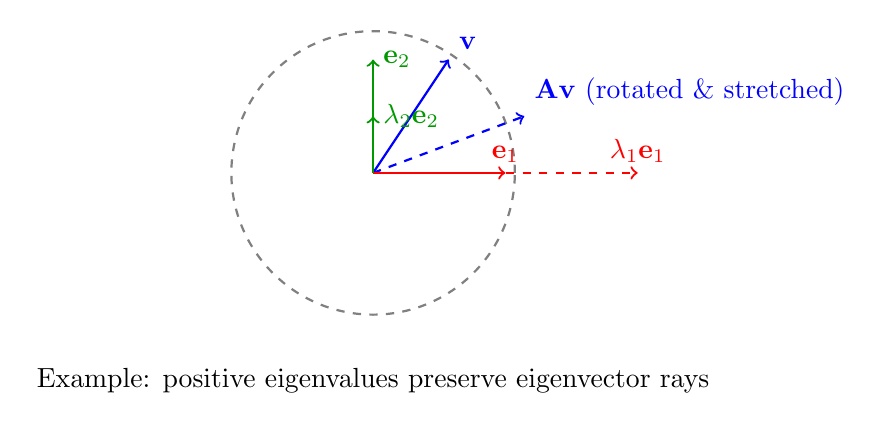
\begin{tikzpicture}[scale=1.2]
  % Circle (unit vectors)
  \draw[gray,dashed,thick] (0,0) circle (1.5cm);

  % Generic vector (rotated and stretched)
  \draw[->,blue,thick] (0,0) -- (0.8,1.2) node[anchor=south west] {$\mathbf{v}$};
  \draw[->,blue,thick,dashed] (0,0) -- (1.6,0.6) node[anchor=south west] {$\mathbf{A}\mathbf{v}$ (rotated \& stretched)};

  % Eigenvector 1 (stretched only, not rotated)
  \draw[->,red,thick] (0,0) -- (1.4,0) node[anchor=south] {$\mathbf{e}_1$};
  \draw[->,red,thick,dashed] (0,0) -- (2.8,0) node[anchor=south] {$\lambda_1 \mathbf{e}_1$};

  % Eigenvector 2 (shrunk, not rotated)
  \draw[->,green!60!black,thick] (0,0) -- (0,1.2) node[anchor=west] {$\mathbf{e}_2$};
  \draw[->,green!60!black,thick,dashed] (0,0) -- (0,0.6) node[anchor=west] {$\lambda_2 \mathbf{e}_2$};

  \node at (0,-2.2) {Example: positive eigenvalues preserve eigenvector rays};
\end{tikzpicture}
\caption{Eigenvectors and a Generic Vector Under $\mathbf A=\operatorname{diag}(2,1/2)$}
\label{fig:eigenvector_geometry}
\end{figure}

\subsection{The Eigenvalue Equation}
\label{subsec:eigen_equation}

\begin{definition}{Eigenvalues and Eigenvectors\index{Eigenvalue}\index{Eigenvector}}{eigenvalue}
Given a square matrix $\mathbf{M} \in \Reals^{n \times n}$, a nonzero vector $\mathbf{v} \in \mathbb C^n$ is called an \emph{eigenvector} of $\mathbf{M}$ if there exists a scalar $\lambda\in\mathbb C$ such that:
\begin{equation}
\label{eq:eigenvalue_equation}
   \mathbf{M}\mathbf{v} = \lambda \mathbf{v}
\end{equation}
The scalar $\lambda$ is the corresponding \emph{eigenvalue}. The requirement that $\mathbf{v} \neq \mathbf{0}$ is essential; otherwise the equation would be trivially satisfied for any $\lambda$.
\end{definition}

\subsubsection{Deriving the Characteristic Polynomial}

How do we actually find the eigenvalues? We rearrange Equation~\eqref{eq:eigenvalue_equation}:
\begin{equation}
    \mathbf{M}\mathbf{v} - \lambda \mathbf{v} = \mathbf{0} \quad \implies \quad (\mathbf{M} - \lambda \mathbf{I})\mathbf{v} = \mathbf{0}
\end{equation}
where $\mathbf{I}$ is the $n \times n$ identity matrix. For a nonzero solution $\mathbf{v}$ to exist, the matrix $(\mathbf{M} - \lambda \mathbf{I})$ must be singular. By our earlier discussion, this means its determinant must vanish:
\begin{equation}
\label{eq:characteristic_polynomial}
    \det(\mathbf{M} - \lambda \mathbf{I}) = 0
\end{equation}
This is the \textbf{characteristic equation}\index{Characteristic Equation}. Expanding the determinant produces a polynomial of degree $n$ in $\lambda$, called the \textbf{characteristic polynomial}. By the Fundamental Theorem of Algebra, this polynomial has exactly $n$ roots (counted with multiplicity, possibly complex), giving us $n$ eigenvalues.

\begin{example}{Computing Eigenvalues of a \texorpdfstring{$2 \times 2$}{2x2} Matrix}{eigen_2x2}
Consider the dynamics matrix of a simple spring system:
\begin{equation}
    \mathbf{A} = \begin{bmatrix} 0 & 1 \\ -4 & -5 \end{bmatrix}
\end{equation}

\textbf{Step 1:} Form $\mathbf{A} - \lambda \mathbf{I}$:
\begin{equation}
    \mathbf{A} - \lambda \mathbf{I} = \begin{bmatrix} -\lambda & 1 \\ -4 & -5 - \lambda \end{bmatrix}
\end{equation}

\textbf{Step 2:} Compute the determinant and set it to zero:
\begin{align}
    \det(\mathbf{A} - \lambda \mathbf{I}) &= (-\lambda)(-5 - \lambda) - (1)(-4) \\
    &= \lambda^2 + 5\lambda + 4 \\
    &= (\lambda + 1)(\lambda + 4) = 0
\end{align}

\textbf{Step 3:} The eigenvalues are $\lambda_1 = -1$ and $\lambda_2 = -4$. Both are negative, meaning this system is \textbf{asymptotically stable}---any perturbation decays exponentially back to equilibrium. The mode associated with $\lambda_1 = -1$ decays slowly (time constant $\tau_1 = 1$ second), while the mode associated with $\lambda_2 = -4$ decays four times faster ($\tau_2 = 0.25$ seconds).

\textbf{Step 4:} Find the eigenvectors. For $\lambda_1 = -1$, solve $(\mathbf{A} + \mathbf{I})\mathbf{v}_1 = \mathbf{0}$:
\begin{equation}
    \begin{bmatrix} 1 & 1 \\ -4 & -4 \end{bmatrix} \mathbf{v}_1 = \mathbf{0} \quad \implies \quad \mathbf{v}_1 = \begin{bmatrix} 1 \\ -1 \end{bmatrix}
\end{equation}
For $\lambda_2 = -4$, solve $(\mathbf{A} + 4\mathbf{I})\mathbf{v}_2 = \mathbf{0}$:
\begin{equation}
    \begin{bmatrix} 4 & 1 \\ -4 & -1 \end{bmatrix} \mathbf{v}_2 = \mathbf{0} \quad \implies \quad \mathbf{v}_2 = \begin{bmatrix} 1 \\ -4 \end{bmatrix}
\end{equation}
\end{example}

\subsection{Physical Interpretation of Eigenvalues}
\label{subsec:eigen_physical}

\begin{enumerate}
    \item \textbf{Inertia tensors and principal axes.} The symmetric rotational inertia tensor about the centre of mass has orthogonal principal axes and corresponding principal moments. For an isolated rigid body with three distinct principal moments, steady torque-free rotation about the intermediate axis is unstable, whereas the minimum and maximum axes are stable to small rotational perturbations. An eigenvector of inertia alone does not establish stability under applied torques, damping or feedback.
    \item \textbf{Constant linear dynamics.} For $\dot{\mathbf x}=A\mathbf x$, all eigenvalues strictly in the open left half-plane imply exponential asymptotic stability. Any eigenvalue with positive real part implies instability. With all real parts nonpositive, stability additionally requires each eigenvalue on the imaginary axis to be semisimple: its Jordan blocks must have size one. Such modes need not decay.
    \item \textbf{Nonlinear and time-varying systems.} At an equilibrium of a continuously differentiable autonomous system, a Hurwitz linearization establishes local exponential stability, and an eigenvalue with positive real part establishes instability. A zero real part can be inconclusive: $\dot x=-x^3$ and $\dot x=x^3$ have the same zero linearization and opposite stability. Instantaneous eigenvalues of a time-varying matrix are not a substitute for its state-transition operator.
\end{enumerate}

For example,
\[
A_0=\begin{pmatrix}0&1\\0&0\end{pmatrix},
\qquad e^{tA_0}\begin{pmatrix}0\\1\end{pmatrix}
=\begin{pmatrix}t\\1\end{pmatrix}
\]
is unbounded despite two zero eigenvalues. By contrast, $A=0$ has bounded constant solutions.

Even negative eigenvalues do not guarantee monotone decrease in a chosen norm. For
\[
A=\begin{pmatrix}-1&10\\0&-1\end{pmatrix},
\qquad
e^{tA}=e^{-t}\begin{pmatrix}1&10t\\0&1\end{pmatrix},
\]
the initial vector $(0,1)^T$ has norm $\sqrt{101}/e>3.6$ at $t=1$ before eventually decaying. The transient comes from the nonorthogonal modal structure. Mixed physical units require a declared metric before interpreting its magnitude. For a fixed positive-definite $P$, the quadratic rate is
\[
\frac{d}{dt}(\mathbf x^TP\mathbf x)
=\mathbf x^T(A^TP+PA)\mathbf x.
\]
Asymptotic stability and short-horizon amplification answer different questions in a finite swing.

\begin{example}{Visualizing Eigenvectors: The Stretching Rubber Sheet}{visualize_eigenvectors}
A general invertible planar map sends a unit circle to an ellipse. Its output axes are \emph{left singular vectors}, while the corresponding input directions are right singular vectors. They need not be the same directions.

The shear
\[
S=\begin{pmatrix}1&1\\0&1\end{pmatrix}
\]
has eigenvalues $1,1$ but singular values $(1+\sqrt5)/2$ and $(\sqrt5-1)/2$. It stretches and contracts different directions even though both eigenvalues are one.

For a symmetric matrix one can choose an orthonormal eigenbasis. The image of the unit ball has semiaxis lengths $|\lambda_i|$; a negative eigenvalue also reverses its eigenvector, and zero gives a collapsed direction. For a positive-definite symmetric matrix the semiaxis lengths equal the positive eigenvalues. This is the special case in which the rubber-sheet picture directly matches the eigenvalue magnitudes.

\end{example}

\subsection{The Spectral Theorem for Symmetric Matrices}
\label{subsec:spectral_theorem}

Among all matrices, \emph{symmetric} matrices ($\mathbf{M} = \mathbf{M}^T$) occupy a privileged position. They arise naturally throughout mechanics (mass matrices, stiffness matrices, inertia tensors) and control theory (cost matrices, Lyapunov functions).

\begin{theorem}{The Spectral Theorem\index{Spectral Theorem}}{spectral}
If $\mathbf{M} \in \Reals^{n \times n}$ is symmetric ($\mathbf{M} = \mathbf{M}^T$), then:
\begin{enumerate}[label=(\roman*)]
    \item All eigenvalues of $\mathbf{M}$ are real.
    \item Eigenvectors corresponding to distinct eigenvalues are orthogonal.
    \item $\mathbf{M}$ can be factored as $\mathbf{M} = \mathbf{Q} \boldsymbol{\Lambda} \mathbf{Q}^T$, where $\mathbf{Q}$ is an orthogonal matrix ($\mathbf{Q}^T\mathbf{Q} = \mathbf{I}$) whose columns are the eigenvectors, and $\boldsymbol{\Lambda} = \text{diag}(\lambda_1, \ldots, \lambda_n)$ is a diagonal matrix of eigenvalues.
\end{enumerate}
\end{theorem}

\begin{proof}[Proof that eigenvalues of a real symmetric matrix are real]
Let $\mathbf M$ be real symmetric. Suppose $\mathbf M\mathbf v=\lambda\mathbf v$ with $\mathbf v\ne0$, allowing complex entries. We will show that $\lambda$ must be real.

Take the complex conjugate transpose (denoted by $^*$) of both sides of $\mathbf{M}\mathbf{v} = \lambda \mathbf{v}$:
\begin{equation}
    \mathbf{v}^* \mathbf{M}^T = \bar{\lambda} \, \mathbf{v}^*
\end{equation}
Since $\mathbf{M} = \mathbf{M}^T$ (and $\mathbf{M}$ is real, so $\mathbf{M}^* = \mathbf{M}^T = \mathbf{M}$):
\begin{equation}
    \mathbf{v}^* \mathbf{M} = \bar{\lambda} \, \mathbf{v}^*
\end{equation}

Now multiply the original equation on the left by $\mathbf{v}^*$:
\begin{equation}
    \mathbf{v}^* \mathbf{M} \mathbf{v} = \lambda \, \mathbf{v}^* \mathbf{v}
\end{equation}
And multiply the conjugated equation on the right by $\mathbf{v}$:
\begin{equation}
    \mathbf{v}^* \mathbf{M} \mathbf{v} = \bar{\lambda} \, \mathbf{v}^* \mathbf{v}
\end{equation}

Equating the right-hand sides:
\begin{equation}
    \lambda \, \mathbf{v}^* \mathbf{v} = \bar{\lambda} \, \mathbf{v}^* \mathbf{v}
\end{equation}

Since $\mathbf{v} \neq \mathbf{0}$, we have $\mathbf{v}^* \mathbf{v} = \sum_i |v_i|^2 > 0$. Dividing both sides by $\mathbf{v}^*\mathbf{v}$ yields $\lambda = \bar{\lambda}$, which is true if and only if $\lambda$ is real.
\end{proof}

\begin{proof}[Proof of Orthogonality for Distinct Eigenvalues]
For real symmetric $\mathbf M$, choose real eigenvectors with distinct eigenvalues:
\[
\mathbf M\mathbf v_1=\lambda_1\mathbf v_1,\qquad
\mathbf M\mathbf v_2=\lambda_2\mathbf v_2,\qquad\lambda_1\ne\lambda_2.
\]
Compute:
\begin{equation}
    \lambda_1 (\mathbf{v}_1^T \mathbf{v}_2) = (\mathbf{M}\mathbf{v}_1)^T \mathbf{v}_2 = \mathbf{v}_1^T \mathbf{M}^T \mathbf{v}_2 = \mathbf{v}_1^T \mathbf{M} \mathbf{v}_2 = \mathbf{v}_1^T (\lambda_2 \mathbf{v}_2) = \lambda_2 (\mathbf{v}_1^T \mathbf{v}_2)
\end{equation}
Therefore $(\lambda_1 - \lambda_2)(\mathbf{v}_1^T \mathbf{v}_2) = 0$. Since $\lambda_1 \neq \lambda_2$, we must have $\mathbf{v}_1^T \mathbf{v}_2 = 0$. The eigenvectors are orthogonal.
\end{proof}

The spectral decomposition $\mathbf M=\mathbf Q\boldsymbol\Lambda\mathbf Q^T$ applies an orthogonal coordinate change to eigenvector axes, scales each coordinate by its eigenvalue, and applies the inverse orthogonal change. Negative eigenvalues reverse signs. Unlike the SVD's nonnegative singular scaling, this diagonal scaling retains the eigenvalue signs.

\subsection{Quadratic Forms and Positive Definiteness}
\label{subsec:quadratic_forms}

In optimization and energy mechanics, we frequently encounter \emph{quadratic forms}\index{Quadratic Form}---scalar-valued functions that are quadratic in a vector argument:

\begin{definition}{Quadratic Form}{quadratic_form}
Given a symmetric matrix $\mathbf{M} \in \Reals^{n \times n}$, the associated \emph{quadratic form} is the scalar function $q: \Reals^n \to \Reals$ defined by:
\begin{equation}
    q(\mathbf{x}) = \mathbf{x}^T \mathbf{M} \mathbf{x} = \sum_{i=1}^n \sum_{j=1}^n M_{ij} \, x_i \, x_j
\end{equation}
\end{definition}

Quadratic forms appear throughout this text series:
\begin{itemize}
    \item \textbf{Kinetic energy:} $T = \frac{1}{2}\dot{\mathbf{q}}^T \mathbf{M}(\mathbf{q}) \dot{\mathbf{q}}$, where $\mathbf{M}(\mathbf{q})$ is the mass matrix (Chapter~\ref{ch:lagrangian}).
    \item \textbf{Optimal control running cost:} $\ell = \mathbf{x}^T \mathbf{Q} \mathbf{x} + \mathbf{u}^T \mathbf{R} \mathbf{u}$, where $\mathbf{Q}$ penalizes state deviations and $\mathbf{R}$ penalizes control effort.
    \item \textbf{Lyapunov functions:} $V(\mathbf{x}) = \mathbf{x}^T \mathbf{P} \mathbf{x}$, used to prove stability (Volume I).
    \item \textbf{Contraction metrics:} $\delta\mathbf{x}^T \mathbf{M}(x) \, \delta\mathbf{x}$, measuring squared infinitesimal length on manifolds (Volume I).
\end{itemize}

\begin{definition}{Positive Definiteness\index{Positive Definite}}{positive_definite}
A symmetric matrix $\mathbf{M}$ is called:
\begin{itemize}
    \item \textbf{Positive definite} ($\mathbf{M} \succ 0$) if $\mathbf{x}^T \mathbf{M} \mathbf{x} > 0$ for all $\mathbf{x} \neq \mathbf{0}$.
    \item \textbf{Positive semi-definite} ($\mathbf{M} \succeq 0$) if $\mathbf{x}^T \mathbf{M} \mathbf{x} \geq 0$ for all $\mathbf{x}$.
    \item \textbf{Negative definite} ($\mathbf{M} \prec 0$) if $\mathbf{x}^T \mathbf{M} \mathbf{x} < 0$ for all $\mathbf{x} \neq \mathbf{0}$.
    \item \textbf{Indefinite} if $\mathbf{x}^T \mathbf{M} \mathbf{x}$ takes both positive and negative values.
\end{itemize}
\end{definition}

\begin{proposition}
\label{prop:pd_eigenvalues}
A symmetric matrix $\mathbf{M}$ is positive definite if and only if all of its eigenvalues are strictly positive.
\end{proposition}

\begin{proof}
By the Spectral Theorem (Theorem~\ref{thm:spectral}), $\mathbf{M} = \mathbf{Q}\boldsymbol{\Lambda}\mathbf{Q}^T$ where $\boldsymbol{\Lambda} = \text{diag}(\lambda_1, \ldots, \lambda_n)$ and $\mathbf{Q}$ is orthogonal. For any nonzero $\mathbf{x}$, define $\mathbf{y} = \mathbf{Q}^T \mathbf{x}$. Since $\mathbf{Q}$ is invertible and $\mathbf{x} \neq \mathbf{0}$, we have $\mathbf{y} \neq \mathbf{0}$. Then:
\begin{equation}
    \mathbf{x}^T \mathbf{M} \mathbf{x} = \mathbf{x}^T \mathbf{Q}\boldsymbol{\Lambda}\mathbf{Q}^T \mathbf{x} = \mathbf{y}^T \boldsymbol{\Lambda} \mathbf{y} = \sum_{i=1}^n \lambda_i y_i^2
\end{equation}

$(\Rightarrow)$ If $\mathbf{M} \succ 0$, then for each eigenvector $\mathbf{v}_i$ (which is nonzero): $\mathbf{v}_i^T \mathbf{M} \mathbf{v}_i = \lambda_i \norm{\mathbf{v}_i}^2 > 0$, so $\lambda_i > 0$.

$(\Leftarrow)$ If all $\lambda_i > 0$ and $\mathbf{y} \neq \mathbf{0}$, then at least one $y_i \neq 0$, so $\sum_i \lambda_i y_i^2 > 0$.
\end{proof}

\begin{laymansbox}{Why Positive Definiteness Matters for Control}{pd_control}
Let the origin be an equilibrium and $V(\mathbf x)=\mathbf x^TP\mathbf x$ with $P\succ0$. Nonincrease of $V$ along solutions gives a stability bound on a suitable invariant neighborhood; it does not imply convergence. An undamped oscillator has constant positive energy and never comes to rest. A negative-definite derivative, with the usual autonomous-system regularity and domain hypotheses, gives asymptotic convergence; a merely semidefinite derivative needs an additional invariant-set argument. $V$ is a mathematical measure and need not be physical energy. Time-varying or global conclusions require their corresponding uniformity, domain and growth assumptions.

\end{laymansbox}

\subsubsection{The Cholesky Decomposition}

A practical consequence of positive definiteness: any positive definite matrix $\mathbf{M}$ can be uniquely factored as:
\begin{equation}
    \mathbf{M} = \mathbf{L}\mathbf{L}^T
\end{equation}
where $\mathbf{L}$ is a lower triangular matrix with strictly positive diagonal entries. This is the \textbf{Cholesky decomposition}\index{Cholesky Decomposition}. It is numerically efficient (roughly half the cost of a general $LU$ factorization) and is the standard method for solving linear systems involving positive definite matrices in physics engines. One usually solves the system rather than explicitly forming its inverse. MuJoCo's documented implementation uses a sparse $L^TDL$ factorization of joint-space inertia and back-substitution; this is related to, but not literally the displayed $LL^T$ algorithm.\footnote{\url{https://mujoco.readthedocs.io/en/stable/computation/index.html}}

For a real symmetric input in exact arithmetic, Cholesky succeeds with strictly positive pivots precisely when the input is positive definite. In floating-point arithmetic, failure can also reflect rounding near the definiteness boundary, incorrect symmetry/storage assumptions or numerical scaling; inspect the data and residual before interpreting it physically. A routine that reads only one triangle does not by itself verify symmetry of the supplied array.

% ------------------------------------------------------------------
\section{The Singular Value Decomposition (SVD)}
\label{sec:svd}
% ------------------------------------------------------------------

What if a matrix is not square? What if it does not have a full set of eigenvectors? The \textbf{Singular Value Decomposition}\index{Singular Value Decomposition} (SVD) is the ultimate, universal factorization of \emph{any} matrix $\mathbf{M} \in \Reals^{n \times m}$, regardless of its shape or rank.

\begin{theorem}{The Singular Value Decomposition}{svd}
Every matrix $\mathbf{M} \in \Reals^{n \times m}$ can be factored as:
\begin{equation}
    \mathbf{M} = \mathbf{U} \boldsymbol{\Sigma} \mathbf{V}^T
\end{equation}
where:
\begin{itemize}
    \item $\mathbf{U} \in \Reals^{n \times n}$ is an orthogonal matrix ($\mathbf{U}^T\mathbf{U} = \mathbf{I}$). Its columns are called the \emph{left singular vectors}.
    \item $\boldsymbol{\Sigma} \in \Reals^{n \times m}$ is a diagonal matrix with non-negative entries $\sigma_1 \geq \sigma_2 \geq \cdots \geq \sigma_{\min(n,m)} \geq 0$ on the diagonal. These are the \emph{singular values}\index{Singular Value}.
    \item $\mathbf{V} \in \Reals^{m \times m}$ is an orthogonal matrix. Its columns are the \emph{right singular vectors}.
\end{itemize}
\end{theorem}

\subsection{Derivation of the SVD From the Eigendecomposition}
\label{subsec:svd_derivation}

The SVD can be derived from the spectral theorem applied to related symmetric matrices. Here is the construction:

\textbf{Step 1.} Form the symmetric matrix $\mathbf{M}^T\mathbf{M} \in \Reals^{m \times m}$. This matrix is always positive semi-definite because for any $\mathbf{x}$:
\begin{equation}
    \mathbf{x}^T (\mathbf{M}^T\mathbf{M}) \mathbf{x} = (\mathbf{M}\mathbf{x})^T (\mathbf{M}\mathbf{x}) = \norm{\mathbf{M}\mathbf{x}}^2 \geq 0
\end{equation}

\textbf{Step 2.} By the Spectral Theorem, $\mathbf{M}^T\mathbf{M}$ has an eigendecomposition:
\begin{equation}
    \mathbf{M}^T\mathbf{M} = \mathbf{V} \boldsymbol{\Lambda} \mathbf{V}^T
\end{equation}
where $\boldsymbol{\Lambda} = \text{diag}(\lambda_1, \ldots, \lambda_m)$ with $\lambda_i \geq 0$ (since $\mathbf{M}^T\mathbf{M}$ is positive semi-definite). Order these eigenvalues decreasingly and take their square roots. Only $\min(n,m)$ singular values are listed in the rectangular diagonal $\Sigma$; when $m>n$, the remaining eigenvalues of $M^TM$ are necessarily zero.

\textbf{Step 3.} For each nonzero singular value $\sigma_i$, define the corresponding left singular vector:
\begin{equation}
    \mathbf{u}_i = \frac{1}{\sigma_i} \mathbf{M} \mathbf{v}_i
\end{equation}
These vectors are orthonormal (a straightforward verification using $\mathbf{M}^T\mathbf{M}\mathbf{v}_i = \sigma_i^2 \mathbf{v}_i$).

\textbf{Step 4.} Extend $\{\mathbf{u}_1, \ldots, \mathbf{u}_r\}$ to a complete orthonormal basis for $\Reals^n$ (where $r = \text{rank}(\mathbf{M})$). Assemble these into the columns of $\mathbf{U}$. Then $\mathbf{M} = \mathbf{U}\boldsymbol{\Sigma}\mathbf{V}^T$ follows by construction. This is an existence proof, not a recommendation to form $M^TM$ numerically: doing so squares the condition number in the full-column-rank case and can obscure small singular values.

\subsection{Geometric Interpretation of the SVD}

The SVD reveals that \emph{any} linear transformation, no matter how complex, can be decomposed into exactly three simple geometric operations:
\begin{enumerate}
    \item \textbf{Reorient the input space by a rotation or reflection} (apply $\mathbf{V}^T$): align the input with the principal directions.
    \item \textbf{Scale each axis independently} (apply $\boldsymbol{\Sigma}$): stretch or shrink along each principal direction.
    \item \textbf{Reorient the output space by a rotation or reflection} (apply $\mathbf{U}$): reorient the result in the output space.
\end{enumerate}

The image of the unit ball is a solid, possibly degenerate ellipsoid in the output space. Rank loss collapses some dimensions; for a rectangular map, the image of a sphere need not be only an ellipsoid's boundary. The singular values are the semi-axis lengths of this ellipsoid, and the left singular vectors point along the ellipsoid's principal axes.

\subsection{The Condition Number}
\label{subsec:condition_number}

For a nonzero, full-rank rectangular matrix, its 2-norm condition number is
\[
\kappa_2(M)=\frac{\sigma_{\max}}{\sigma_{\min}},
\]
where the denominator is the smallest of the $\min(n,m)$ listed singular values. Rank deficiency is conventionally assigned infinite condition number here. A wide, full-row-rank matrix may have finite condition number and a nontrivial input kernel simultaneously.

For a nonsingular square system $M\mathbf x=\mathbf b$ with fixed $M$ and nonzero $\mathbf b$, the relative perturbation bound is
\[
\frac{\|\delta\mathbf x\|_2}{\|\mathbf x\|_2}
\le \kappa_2(M)\frac{\|\delta\mathbf b\|_2}{\|\mathbf b\|_2}.
\]
Absolute inverse gain is instead $\|M^{-1}\|_2=1/\sigma_{\min}$. For $M=10^{-3}I$, the condition number is one but the absolute inverse gain is 1000. Forward gain is $\sigma_{\max}$, not the condition number. Matrix perturbations and general least-squares problems need additional bounds.

Singular values depend on coordinate units and chosen norms. A task Jacobian mixing translation and rotation, or joint coordinates measured in degrees rather than radians, needs explicit scaling or a metric before its condition number is a physical comparison.

\subsection{Truncated SVD and Low-Rank Approximation}

One of the most powerful applications of the SVD is data compression. Given a matrix $\mathbf{M}$ with singular values $\sigma_1 \geq \sigma_2 \geq \cdots$, the best rank-$k$ approximation (in the Frobenius norm) is:
\begin{equation}
    \mathbf{M}_k = \sum_{i=1}^k \sigma_i \, \mathbf{u}_i \mathbf{v}_i^T
\end{equation}
This result (the Eckart-Young-Mirsky theorem) underpins dimensionality reduction techniques like Principal Component Analysis (PCA), which identifies the dominant modes of variation in high-dimensional data such as motion capture recordings of golf swings.

\begin{example}{The SVD of the Jacobian (Manipulability Ellipsoid)}{svd_jacobian}
For seven independent joint velocities and a three-dimensional hand-position task, $J\in\Reals^{3\times7}$ maps $\dot{\mathbf q}$ to $\mathbf v_H$. With the declared budget $\|\dot{\mathbf q}\|_2\le1$:
\begin{itemize}
    \item The columns of $U$ are task-space singular directions. A direction with zero singular value is absent from the instantaneous velocity image.
    \item The three singular values give the semiaxes of the image of that joint-speed ball. They are not actual maximum speeds without this budget, its units and actuator feasibility.
    \item The columns of $V$, not of $V^T$, give the corresponding joint-velocity directions. Its remaining columns span the input kernel.
\end{itemize}

For a positive-definite joint-speed metric $H$ and task metric $W$, normalize the map as
\[
\widetilde J=W^{1/2}JH^{-1/2},
\qquad \dot{\mathbf q}^TH\dot{\mathbf q}\le1.
\]
Singular values of this normalized map compare declared physical budgets; unscaled Euclidean values need not survive a change of units.

Virtual work gives $\boldsymbol\tau=J^T\mathbf F$ and power equality $\boldsymbol\tau^T\dot{\mathbf q}=\mathbf F^T\mathbf v_H$. Under the dual torque budget $\boldsymbol\tau^TH^{-1}\boldsymbol\tau\le1$, feasible quasistatic task forces satisfy
\[
\mathbf F^TJH^{-1}J^T\mathbf F\le1.
\]
At full row rank this gives reciprocal force/velocity semiaxes in consistent normalized coordinates. At rank loss it may be unbounded in a task-force direction supported by ideal constraints. It does not predict unlimited real force: structural strength, joint/contact limits, compliance, actuation, balance and dynamics still matter.
\end{example}

\subsection{Instantaneous Rank and Finite-Time Control}

A full-row-rank $3\times7$ task Jacobian has a four-dimensional kernel without being singular. More generally, a kinematic singularity is a drop below the maximum rank attainable by the specified mechanism and task; an inherently lower-dimensional image is not itself evidence of a singular configuration. This kinematic redundancy differs from underactuation, which concerns the rank and admissible set of the actuator map in the dynamics.

Initial task-null velocity also need not preserve finite position. For two unit planar links,
\[
\mathbf p(\mathbf q)=
\begin{pmatrix}\cos q_1+\cos(q_1+q_2)\\
\sin q_1+\sin(q_1+q_2)\end{pmatrix},
\]
the straight configuration has $J(0)=\begin{pmatrix}0&0\\2&1\end{pmatrix}$. Its kernel contains $(1,-2)^T$, but the straight coordinate step $\mathbf q(t)=t(1,-2)^T$ gives $\mathbf p(t)=(2\cos t,0)^T$, not a stationary hand.

Conversely, a one-dimensional instantaneous input can control more than one state over time. For the double integrator
\[
A=\begin{pmatrix}0&1\\0&0\end{pmatrix},\qquad
B=\begin{pmatrix}0\\1\end{pmatrix},
\]
$B$ has rank one while $[B,AB]$ has rank two. Its controllability Gramian is
\[
W_c(T)=\begin{pmatrix}T^3/3&T^2/2\\T^2/2&T\end{pmatrix},
\qquad \det W_c(T)=T^4/12>0\quad(T>0).
\]
This unconstrained linear result does not remove finite torque bounds or contact requirements. It shows why instantaneous rank, finite-time reachability, observation and a successful golf delivery must be evaluated using their respective maps and assumptions.

Observation has the same temporal distinction. If position alone is measured, $C=[1,0]$ has an instantaneous kernel containing velocity. Yet the observability matrix $\mathcal O=[C^T,(CA)^T]^T=I_2$ has full rank: position measurements over time reveal velocity in this ideal model. A kernel of $C$ is not necessarily an unobservable dynamical subspace.

% ==================================================================
%  Section: Dyads, Dyadics, and Tensor Products
% ==================================================================

\section{Dyads, Dyadics, and Tensor Products}
\label{sec:dyads-dyadics}

The matrix decompositions we have studied so far---eigendecomposition,
SVD---break a matrix into pieces that reveal its geometric action.
In this section we meet a complementary idea: building matrices up
from the simplest possible pieces, called \emph{dyads}.
This viewpoint is not merely algebraic; it is the language that
mechanics has used for over a century to describe inertia, stress,
and stiffness without ever choosing a coordinate frame~\cite{Murray1994}.

% ------------------------------------------------------------------
\subsection{What Is a Dyad?}
\label{subsec:dyad-definition}

\begin{definition}{\texorpdfstring{Dyad (Outer Product)}{Dyad (Outer Product)}}{dyad}
Given two vectors $\mathbf{a}\in\Reals^{m}$ and
$\mathbf{b}\in\Reals^{n}$, the \textbf{dyad}\index{dyad}
(or \textbf{outer product}\index{outer product}) is the
$m\times n$ matrix
\[
  \mathbf{D} \;=\; \mathbf{a}\,\mathbf{b}^{T}.
\]
This matrix has rank at most one: every column is a scalar multiple
of $\mathbf{a}$, and every row is a scalar multiple of $\mathbf{b}^{T}$.
\end{definition}

A dyad encodes \emph{two} directions simultaneously.
When it acts on a vector $\mathbf{v}$,
\[
  \mathbf{D}\,\mathbf{v}
  \;=\;
  \bigl(\mathbf{a}\,\mathbf{b}^{T}\bigr)\mathbf{v}
  \;=\;
  \mathbf{a}\,\inner{\mathbf{b}}{\mathbf{v}},
\]
it first \emph{senses} how much $\mathbf{v}$ aligns with $\mathbf{b}$
(via the inner product $\inner{\mathbf{b}}{\mathbf{v}}$) and then
\emph{responds} along the direction $\mathbf{a}$, scaled by that
alignment.

\begin{laymansbox}{Dyads: Direction of Action and Direction of Sensitivity}{dyad_intuition}
The dyad $\mathbf a\mathbf b^T$ measures the component of an input along $\mathbf b$ and produces a response along $\mathbf a$. It has rank one if both vectors are nonzero, and rank zero otherwise. This is an algebraic response channel, not automatically a passive spring.

For an unprestressed conservative spring along a unit direction $\mathbf n$, stored energy $\frac12k(\mathbf n^T\mathbf u)^2$ gives restoring force $-k\mathbf n\mathbf n^T\mathbf u$. Its stiffness is symmetric. A generic cross-direction dyad is nonsymmetric and cannot by itself be the Hessian of a smooth elastic potential. For example, the field $(0,x)$ does one unit of work around the positively oriented unit square; a conservative spring would do zero net closed-path work.

\end{laymansbox}

\begin{example}{A Rank-1 Linear Response}{dyad_force}
Let $\mathbf{a} = \begin{bmatrix}0\\1\\0\end{bmatrix}$ (vertical)
and $\mathbf{b} = \begin{bmatrix}1\\0\\0\end{bmatrix}$ (horizontal).
Then
\[
  \mathbf{D}
  = \mathbf{a}\,\mathbf{b}^{T}
  = \begin{bmatrix}0\\1\\0\end{bmatrix}
    \begin{bmatrix}1&0&0\end{bmatrix}
  = \begin{bmatrix}0&0&0\\1&0&0\\0&0&0\end{bmatrix}.
\]
Applied to a displacement
$\mathbf{v}=\begin{bmatrix}3\\5\\2\end{bmatrix}$:
\[
  \mathbf{D}\,\mathbf{v}
  = \begin{bmatrix}0\\3\\0\end{bmatrix}.
\]
The dyad extracts the horizontal component ($3$) and produces a
purely vertical response---exactly the one-channel behaviour
described above.
\end{example}

% ------------------------------------------------------------------
\subsection{From Dyads to Dyadics}
\label{subsec:dyadics}

A nonzero dyad has rank one. Physical stiffness, inertia and stress maps may have full rank or may have null directions.  We get there by \emph{summing} dyads.

\begin{definition}{\texorpdfstring{Dyadic (Tensor Product Expansion)}{Dyadic (Tensor Product Expansion)}}{dyadic}
A \textbf{dyadic}\index{dyadic} is a finite sum of dyads:
\[
  \mathbf{T}
  \;=\;
  \sum_{k=1}^{r} \mathbf{a}_{k}\,\mathbf{b}_{k}^{T}.
\]
Every $m\times n$ matrix can be written in this form with
$r\leq\min(m,n)$ terms.
\end{definition}

This is not a new fact---it is the column--row factorisation you
already know from the SVD\@.  If
$\mathbf{A}=\mathbf{U}\boldsymbol{\Sigma}\mathbf{V}^{T}$, then
\[
  \mathbf{A}
  \;=\;
  \sum_{k=1}^{r}\sigma_{k}\,\mathbf{u}_{k}\,\mathbf{v}_{k}^{T},
\]
which is a dyadic with $r$ terms (the rank of $\mathbf{A}$).  The SVD
merely chooses the \emph{orthogonal} dyad decomposition; infinitely
many other decompositions exist.

Abstractly, a linear map $V\to W$ belongs to $W\otimes V^*$: its input slot is a covector. In standard Euclidean coordinates the inner product identifies $\Reals^n$ with its dual, so $\mathbf a\mathbf b^T$ can be written using two vector coordinate arrays and identified with an elementary tensor in $\Reals^m\otimes\Reals^n$. Under general coordinate changes one must retain which slots are vectors and which are covectors.

% ------------------------------------------------------------------
\subsection{Physical Meaning in Mechanics}
\label{subsec:dyadics-mechanics}

The power of the dyadic viewpoint is that it names the two ``slots''
of a matrix: input direction and output direction.  Three central
objects in mechanics are dyadics.

\paragraph{The Inertia Tensor.}\index{inertia tensor}
About the centre of mass, the rotational inertia of a rigid body maps angular velocity to angular momentum:
\begin{equation}\label{eq:inertia-dyadic-map}
  \mathbf{L} \;=\; \mathbf{I}\,\boldsymbol{\omega}.
\end{equation}
Here $\boldsymbol{\omega}$ is the ``input'' (the axis and rate of
spin) and $\mathbf{L}$ is the ``output'' (the direction and magnitude
of angular momentum).  For a generic direction in a body with unequal principal moments,
$\mathbf{L}$ and $\boldsymbol{\omega}$ need not be parallel; they are parallel along every principal axis even without an isotropic inertia;
the inertia tensor is the dyadic that encodes this directional coupling.

\paragraph{The Stress Tensor.}\index{stress tensor}
The Cauchy stress tensor $\boldsymbol{\sigma}$ maps a surface-normal
direction $\hat{\mathbf{n}}$ to the traction (force per unit area)
$\mathbf{t}$ acting on that surface:
\[
  \mathbf{t} \;=\; \boldsymbol{\sigma}\,\hat{\mathbf{n}}.
\]
Input: the orientation of a small area element.  Output: the force
that the material on one side exerts on the other.

\paragraph{The Stiffness Matrix.}\index{stiffness matrix}
For a small-displacement, unprestressed truss, let $\mathbf u$ collect all nodal displacements and $B_e\mathbf u$ be member $e$'s axial extension. The external balancing force is $\mathbf f=K\mathbf u$, with
\[
K=\sum_e k_e B_e^TB_e,\qquad k_e=\frac{E_eA_e}{L_e}.
\]
For a member between two three-dimensional nodes, its nonzero incidence blocks are $B_e=[-\mathbf n_e^T,\mathbf n_e^T]$. Thus one member contributes a rank-one \emph{nodal} matrix, not merely a $3\times3$ direction matrix. A single anchored-node star is a special case in which the free-node stiffness reduces to $\sum_e k_e\mathbf n_e\mathbf n_e^T$.

Unrestrained rigid translations give null modes of the assembled matrix. Prestress, geometric stiffness, constraints and nonlinear deformation require additional terms or a tangent linearization. Summing member directions alone does not encode the connectivity of a general truss.

\begin{laymansbox}{Why Engineers Say ``Tensor''}{tensor_word}
When a mechanical engineer refers to the ``inertia tensor'' or
``stress tensor,'' the usual rigid-body inertia and classical Cauchy stress have symmetric $3\times3$ representations. Symmetry of Cauchy stress here assumes the classical angular-momentum balance without independent couple stresses; not every tensor or linear response is symmetric.  The word \emph{tensor} signals
that the object transforms in a specific, predictable way under
changes of coordinate frame.
It is not just a bag of nine numbers; it is a physical machine that
takes one vector in and produces another vector out, regardless of
how you choose your axes.
\end{laymansbox}

% ------------------------------------------------------------------
\subsection{The Coordinate-Free Perspective}
\label{subsec:coordinate-free}

\index{coordinate-free formulation}
A dyadic is a geometric object that lives in the space of linear maps
$\Reals^{n}\to\Reals^{m}$.  Choosing a basis gives it a matrix
representation, but the underlying map does not depend on that choice.

\begin{example}{Inertia Tensor of a Point Mass}{point_mass_inertia}
A point mass $m$ at displacement $\mathbf r$ from a chosen reference origin contributes
inertia tensor
\begin{equation}\label{eq:point-mass-inertia}
  \mathbf{I}
  \;=\;
  m\bigl(\norm{\mathbf{r}}^{2}\,\mathbf{1}
         - \mathbf{r}\,\mathbf{r}^{T}\bigr),
\end{equation}
where $\mathbf{1}$ is the $3\times3$ identity.  Notice that no
basis vectors appear---$\mathbf{r}\,\mathbf{r}^{T}$ is a dyad
formed from the position vector with itself, and $\mathbf{1}$
is the identity map. This expression is \emph{coordinate-free}: it is valid in every
frame simultaneously.
\end{example}

When we change from a body-fixed frame $\{B\}$ to a world frame
$\{W\}$ via a rotation $\mathbf{R}\in\SO$, the matrix
representation of the inertia tensor transforms by the
\textbf{congruence transformation}\index{congruence transformation}:
\begin{equation}\label{eq:congruence}
  \mathbf{I}^{W}
  \;=\;
  \mathbf{R}\,\mathbf{I}^{B}\,\mathbf{R}^{T}.
\end{equation}
The congruence form $\mathbf{R}\,(\cdot)\,\mathbf{R}^{T}$
rotates both the input slot and the output slot of the dyadic.  It
preserves symmetry, positive-definiteness, and---for rotations---eigenvalues
(the principal moments of inertia). This formula changes orientation about the same reference point; changing the origin also requires the parallel-axis contribution.

% ------------------------------------------------------------------
\subsection{Basis, Metric and Mechanical Duality}

If old velocity coordinates and new coordinates satisfy $\mathbf v=S\widetilde{\mathbf v}$ for an invertible $S$, preservation of kinetic energy and power requires
\[
\widetilde M=S^TMS,\qquad
\widetilde{\boldsymbol\tau}=S^T\boldsymbol\tau,
\]
\[
\widetilde{\mathbf v}^T\widetilde M\widetilde{\mathbf v}
=\mathbf v^TM\mathbf v,\qquad
\widetilde{\boldsymbol\tau}^T\widetilde{\mathbf v}
=\boldsymbol\tau^T\mathbf v.
\]
This congruence law describes the kinetic bilinear form and its vector-to-covector map. A linear endomorphism instead has the similarity law $\widetilde A=S^{-1}AS$. For an orthogonal $S$, the two transformation patterns can look alike, which can hide the distinction.

Congruence preserves definiteness but generally changes ordinary matrix eigenvalues. Physical comparisons in nonorthogonal or differently scaled coordinates require the corresponding metric, not raw eigenvalues or a dot product chosen only because the arrays have equal length. This distinction connects velocity transmission through $J$ to force transmission through $J^T$, and prevents coordinate-dependent numerical norms from being labeled energy or effort without a model.

\subsection{Connection to the Rest of This Book}
\label{subsec:dyadic-connections}

The dyadic point of view recurs throughout our study of rigid-body
mechanics:

\begin{itemize}
  \item \textbf{Screw axes and wrenches (Chapter~5).}
    A wrench combines a force and a moment into a single six-dimensional
    object.  The spatial inertia is a $6\times6$ map from twist to spatial momentum, not directly to wrench. A wrench is related to momentum rate, including the transport terms required by a moving coordinate frame.

  \item \textbf{Spatial algebra (Chapter~8).}
    With twist ordered as $(\boldsymbol\omega,\mathbf v_O)$ and centre-of-mass displacement $\mathbf c$ from the reference origin $O$, the spatial inertia is
    \[
    \mathcal I_O=
    \begin{bmatrix}
    I_O&m[\mathbf c]_\times\\
    -m[\mathbf c]_\times&mI_3
    \end{bmatrix}.
    \]
    Here $I_O$ is rotational inertia about $O$, not about the centre of mass unless the origins coincide. The matrix maps twist to angular momentum about $O$ and linear momentum, and is SPD when every nonzero rigid-body twist has positive kinetic energy. In a body-fixed frame attached to the rigid body,
    $\mathbf w=\mathcal I_O\dot{\mathbf v}+\mathbf v\times^*(\mathcal I_O\mathbf v)$,
    where the force cross-product operator includes the required frame transport. The momentum map itself contains no acceleration.

  \item \textbf{The mass matrix (Chapter~11).}
    The joint-space mass matrix $\mathbf{M}(\mathbf{q})$ that appears
    in the manipulator equation
    $\mathbf{M}\ddot{\mathbf{q}}+\mathbf{c}=\boldsymbol{\tau}$
    is a configuration-dependent dyadic on joint-velocity space.
    Each link contributes a term built from Jacobians and spatial
    inertias through $M(\mathbf q)=\sum_i J_i^T\mathcal I_iJ_i$, with each twist Jacobian and inertia expressed about matching origins in matching frames. This is the kinetic-energy counterpart of assembling nodal stiffness through a compatibility map.

  \item \textbf{The articulated-body algorithm (Chapter~10).}
    Featherstone's algorithm propagates \emph{articulated-body inertias}
    through a kinematic tree.  These are $6\times6$ dyadics that
    account for the coupling between a link's motion and the
    reactions of all its descendants.
\end{itemize}

Understanding that all these objects are dyadics---linear maps built
from sums of outer products---provides a unifying thread: the same
algebraic structure appears whether we are analysing a truss, spinning
a gyroscope, or computing the forward dynamics of a humanoid robot.

% ==================================================================
%  Section: Matrix Norms and Conditioning
% ==================================================================

\section{Matrix Norms and Conditioning}
\label{sec:matrix_norms}

\index{matrix norm}
Having decomposed matrices via the eigendecomposition and SVD, we now turn
to a fundamental practical question: \emph{how large is a matrix, and how
sensitive is a linear system to perturbations?}  Matrix norms quantify the
first question; the \emph{condition number} answers the second.

\begin{definition}{\texorpdfstring{Frobenius Norm $\norm{\mathbf{A}}_F$}{Frobenius Norm}}{frobenius_norm}
The \textbf{Frobenius norm}\index{Frobenius norm} of a matrix
$\mathbf{A}\in\Reals^{m\times n}$ is
\begin{equation}
  \label{eq:frobenius_norm}
  \norm{\mathbf{A}}_F
  \;=\; \sqrt{\sum_{i=1}^{m}\sum_{j=1}^{n} a_{ij}^{2}}
  \;=\; \sqrt{\operatorname{tr}\!\bigl(\mathbf{A}^{T}\mathbf{A}\bigr)}
  \;=\; \sqrt{\sigma_1^{2}+\sigma_2^{2}+\cdots+\sigma_{\min(m,n)}^{2}}.
\end{equation}
The last equality follows directly from the SVD\@.  The Frobenius norm
treats the matrix as a long vector and computes its Euclidean length.
\end{definition}

\begin{definition}{\texorpdfstring{Spectral Norm $\norm{\mathbf{A}}_2$}{Spectral Norm}}{spectral_norm}
The \textbf{spectral norm}\index{spectral norm} (also called the
\emph{operator 2-norm} or \emph{induced 2-norm}) is
\begin{equation}
  \label{eq:spectral_norm}
  \norm{\mathbf{A}}_2
  \;=\; \max_{\norm{\mathbf{x}}_2=1} \norm{\mathbf{A}\mathbf{x}}_2
  \;=\; \sigma_{\max}(\mathbf{A}).
\end{equation}
This is the maximum factor by which $\mathbf{A}$ can stretch a unit
vector---exactly the length of the longest semi-axis of the image
ellipsoid from the SVD's geometric interpretation
(Section~\ref{sec:svd}).
\end{definition}

\begin{definition}{\texorpdfstring{Condition Number $\kappa(\mathbf{A})$}{Condition Number}}{condition_number}
\index{condition number}
For a matrix $\mathbf{A}$ with $\sigma_{\min}>0$, the
\textbf{condition number} with respect to the 2-norm is
\begin{equation}
  \label{eq:condition_number}
  \kappa(\mathbf{A})
  \;=\; \frac{\sigma_{\max}}{\sigma_{\min}}.
\end{equation}
When $\sigma_{\min}=0$ (i.e., $\mathbf{A}$ is singular), we define
$\kappa(\mathbf{A})=\infty$.
A well-conditioned matrix has $\kappa\approx 1$; an ill-conditioned
matrix has $\kappa\gg 1$.
\end{definition}

\subsection{What the Pseudoinverse Does Not Guarantee}

For $J=U\Sigma V^T$, the Moore--Penrose pseudoinverse is $J^+=V\Sigma^+U^T$, with each nonzero singular value inverted. The command $J^+\mathbf v$ is the minimum-Euclidean-norm least-squares solution. It exactly realizes $\mathbf v$ only when $\mathbf v\in\operatorname{im}J$; its notion of minimum norm depends on the declared units and metric.

The pseudoinverse does not remove near-singular amplification. With $J=\operatorname{diag}(1,10^{-3})$ and desired velocity $(1,1)^T$, it requests joint velocity $(1,1000)^T$. Error in the weak task direction is amplified; error in every direction need not be. A condition-number threshold alone also misses an overall loss of scale such as $J=\epsilon I$, whose condition number stays one as $\epsilon\to0$.

A damped least-squares alternative solves
\[
\min_{\dot{\mathbf q}}\ \|J\dot{\mathbf q}-\mathbf v\|_2^2
+\lambda^2\|\dot{\mathbf q}\|_2^2,\qquad \lambda>0,
\]
and applies singular-direction gains
\[
\frac{\sigma_i}{\sigma_i^2+\lambda^2}
\le\frac{1}{2\lambda}.
\]
This bounds inverse gain by accepting a task residual. It does not enforce joint-speed limits, contact constraints or closed-loop stability by itself. Truncated SVD likewise requires an explicit tolerance for treating small measured singular values as zero; numerical rank is not automatically exact physical rank.

For a golf model, a small singular value can explain why a chosen hand-velocity correction demands a large joint-velocity change at one configuration. Predicting actual motion additionally requires the inertial equations, actuator limits and controller. Neither shaking nor a beneficial release follows from the condition number alone.

% ==================================================================
%  Section: Matrix Decompositions for Computation
% ==================================================================

\section{Matrix Decompositions for Computation}
\label{sec:matrix_decompositions_computation}

\index{matrix decomposition}
The eigendecomposition and SVD reveal geometric structure.  This section
surveys three additional decompositions whose primary purpose is
\emph{computational efficiency} when solving the linear systems that
arise throughout dynamics and control.

\subsection{LU Decomposition}
\label{subsec:lu_decomposition}
\index{LU decomposition}

Any invertible matrix $\mathbf{A}\in\Reals^{n\times n}$ can (with row
permutations) be factored as
\begin{equation}
  \label{eq:lu_decomposition}
  \mathbf{P}\mathbf{A} = \mathbf{L}\mathbf{U},
\end{equation}
where $\mathbf{P}$ is a permutation matrix, $\mathbf{L}$ is unit lower
triangular, and $\mathbf{U}$ is upper triangular.  Solving
$\mathbf{A}\mathbf{x}=\mathbf{b}$ then reduces to two triangular
solves (forward and back substitution), each costing $O(n^{2})$ after
the $O(n^{3})$ factorization.  When multiple right-hand sides share
the same $\mathbf{A}$, LU is the workhorse: factor once, solve many
times.

\subsection{QR Decomposition}
\label{subsec:qr_decomposition}
\index{QR decomposition}

For any $\mathbf{A}\in\Reals^{m\times n}$ with $m\geq n$,
\begin{equation}
  \label{eq:qr_decomposition}
  \mathbf{A} = \mathbf{Q}\mathbf{R},
\end{equation}
where $\mathbf{Q}\in\Reals^{m\times m}$ is orthogonal and
$\mathbf{R}\in\Reals^{m\times n}$ is upper trapezoidal: an upper-triangular $n\times n$ block above zero rows.
QR is the preferred method for solving least-squares problems
$\min_{\mathbf{x}}\norm{\mathbf{A}\mathbf{x}-\mathbf{b}}_2$ because,
unlike the normal equations $\mathbf{A}^{T}\mathbf{A}\mathbf{x}=
\mathbf{A}^{T}\mathbf{b}$, it avoids squaring the condition number
($\kappa_2(\mathbf{A}^{T}\mathbf{A})=\kappa_2(\mathbf{A})^{2}$ for full column rank). A backward-stable QR solve avoids that additional conditioning penalty. Rank-deficient problems need an appropriate rank-revealing or SVD treatment, particularly when a minimum-norm solution is required.

\subsection{Cholesky Decomposition}
\label{subsec:cholesky_decomposition}
\index{Cholesky decomposition}

If $\mathbf{M}\in\Reals^{n\times n}$ is symmetric positive definite
(SPD), then there exists a unique lower-triangular matrix $\mathbf{L}$
with positive diagonal entries such that
\begin{equation}
  \label{eq:cholesky_decomposition}
  \mathbf{M} = \mathbf{L}\mathbf{L}^{T}.
\end{equation}
Dense Cholesky costs roughly half the leading-order flops of dense LU and is backward stable under the usual floating-point assumptions for a sufficiently well-resolved SPD input. No pivoting is needed in exact arithmetic. Near-singularity, underflow, overflow and loss of definiteness through rounding remain numerical concerns.

\begin{principle}{Cholesky and the Mass Matrix}{cholesky_mass_matrix}
In independent generalized-velocity coordinates, a model with strictly positive kinetic energy for every nonzero admissible velocity has an SPD mass matrix. Redundant embedding coordinates, massless idealizations or singular coordinate charts can violate that premise. With ideal constraints one may instead solve a reduced system or an indefinite saddle-point system; Cholesky does not directly apply to every augmented matrix.

For the unconstrained SPD solve $M\ddot{\mathbf q}=\boldsymbol\tau-\mathbf h-\mathbf g$, Cholesky or a structure-exploiting factorization is appropriate. An articulated-body algorithm can solve tree dynamics recursively without explicitly forming the full dense matrix. Choose the algorithm for the model and sparsity rather than treating one factorization as universal~\cite{nocedal2006}.

\end{principle}

% ------------------------------------------------------------------
\section{Worked Example: Eigenvalue and SVD Analysis in Python}
\label{sec:ch1_python_example}
% ------------------------------------------------------------------

Let us bring together the theory developed in this chapter with a concrete computational example. The following Python code constructs a $3 \times 3$ symmetric matrix (representing a simplified 3D inertia tensor), computes its eigendecomposition and SVD, and verifies the key properties we have proven.

\begin{lstlisting}[language=Python, caption=Eigendecomposition and SVD of a Symmetric Matrix]
import numpy as np

# ---- Define a symmetric positive definite matrix ----
# This could represent a simplified 3D inertia tensor
M = np.array([
    [5.0, 1.0, 0.5],
    [1.0, 4.0, 0.3],
    [0.5, 0.3, 3.0]
])

# Verify symmetry
assert np.allclose(M, M.T), "Matrix is not symmetric!"

# ---- Eigendecomposition ----
eigenvalues, eigenvectors = np.linalg.eigh(M)  # eigh for symmetric matrices
print("Eigenvalues:", np.round(eigenvalues, 4))
print("Eigenvectors (columns):\n", np.round(eigenvectors, 4))

# Positive principal moments plus their triangle inequalities
# are required for a physical three-dimensional inertia tensor.
assert eigenvalues[-1] <= eigenvalues[0] + eigenvalues[1]

# Verify: all eigenvalues positive => positive definite
assert all(eigenvalues > 0), "Matrix is not positive definite!"
print("Matrix is POSITIVE DEFINITE (all eigenvalues > 0)")

# Verify: eigenvectors are orthogonal
QTQ = eigenvectors.T @ eigenvectors
print("Q^T Q (should be identity):\n", np.round(QTQ, 10))

# Verify spectral decomposition: M = Q * Lambda * Q^T
M_reconstructed = eigenvectors @ np.diag(eigenvalues) @ eigenvectors.T
print("Reconstruction error:", np.linalg.norm(M - M_reconstructed))

# ---- Singular Value Decomposition ----
U, sigma, VT = np.linalg.svd(M)
print("\nSingular values:", np.round(sigma, 4))
print("Eigenvalues (sorted descending):", np.round(sorted(eigenvalues, reverse=True), 4))
print("For symmetric PD matrices, singular values = eigenvalues (sorted)")

# ---- Condition Number ----
kappa = sigma[0] / sigma[-1]
print(f"\nCondition number: {kappa:.4f}")
print("(Close to 1 means well-conditioned; >>1 means ill-conditioned)")

# ---- Cholesky Decomposition ----
L = np.linalg.cholesky(M)
print("\nCholesky factor L:\n", np.round(L, 4))
print("Verify L @ L^T = M, error:", np.linalg.norm(M - L @ L.T))
\end{lstlisting}

% ------------------------------------------------------------------
\section{Chapter Summary}
\label{sec:ch1_summary}
% ------------------------------------------------------------------

\begin{principle}{Key Takeaways from Chapter 1}{ch1_summary}
\begin{enumerate}
    \item A \textbf{vector space} is defined by eight axioms guaranteeing closure, commutativity, and compatibility of addition and scalar multiplication. $\Reals^n$ is the prototypical example.

    \item The \textbf{rank} of a matrix counts independent columns; the \textbf{null space} captures the ``lost'' dimensions. The \textbf{Rank-Nullity Theorem} connects them: $\text{rank} + \text{nullity} = \text{number of columns}$.

    \item The \textbf{dot product} measures alignment between vectors and defines orthogonality. The \textbf{cross product} in $\Reals^3$ produces a perpendicular vector and can be written as a \emph{skew-symmetric matrix} multiplication---a representation central to Lie Algebra ($\mathfrak{so}(3)$).

    \item \textbf{Eigenvalues} characterize asymptotic stability of a constant continuous-time linear system, with Jordan structure needed on the imaginary-axis boundary. Eigenvectors of a symmetric inertia tensor give principal axes; its eigenvalues give principal moments. The \textbf{Spectral Theorem} guarantees that symmetric matrices have real eigenvalues and orthogonal eigenvectors.

    \item \textbf{Positive definiteness} ($\mathbf{M} \succ 0$) guarantees a quadratic form has a strict minimum---the cornerstone of Lyapunov stability proofs and energy-based control design.

    \item The \textbf{SVD} decomposes a matrix into orthogonal transformations and nonnegative scaling. Applied to a Jacobian with declared input and output metrics, it describes instantaneous velocity transmission. Relative conditioning, absolute inverse gain and finite-time controllability answer different questions.
\end{enumerate}
\end{principle}

% ------------------------------------------------------------------
\section{Further Reading}
\label{sec:ch1_further_reading}
% ------------------------------------------------------------------

The material in this chapter draws on a long tradition of textbooks at the
intersection of linear algebra and applied mathematics. For a comprehensive
undergraduate treatment that emphasizes geometric intuition alongside
computational technique, Strang~\cite{strang2019} remains the standard
reference; his ``four fundamental subspaces'' perspective directly informs
the rank-nullity discussion presented here.

In the robotics context, Chapter~2 of Murray, Li, and
Sastry~\cite{Murray1994} develops the specific linear-algebraic tools---rotation
matrices, skew-symmetric operators, and the Lie bracket---that recur throughout
the rest of this textbook. Readers who wish to pursue the numerical aspects of
linear algebra, particularly iterative solvers and the role of condition numbers
in optimization, will find Nocedal and Wright~\cite{nocedal2006} an invaluable
companion.

The dyadic and tensor-product viewpoint introduced in
Section~\ref{sec:dyads-dyadics} connects directly to continuum mechanics, where
stress and strain are second-order tensors built from exactly the same outer-product
construction. Students interested in these connections should consult any
graduate text on continuum mechanics or tensor analysis.

Finally, the eigenvalue structures and matrix exponentials introduced in this
chapter are the first hints of \emph{Lie theory}. Hall~\cite{hall2015} provides
a mathematically rigorous bridge from linear algebra to Lie groups and Lie
algebras, foreshadowing the rotation groups ($\SO(3)$) and rigid-body
transformation groups ($\SE(3)$) that appear in Chapters~4 and~5.

% ------------------------------------------------------------------
\section{Exercises}
\label{sec:ch1_exercises}
% ------------------------------------------------------------------

\subsection*{Computational Exercises}

\begin{enumerate}
    \item \textbf{(Rank and Null Space)} Given the matrix
    \begin{equation*}
        \mathbf{A} = \begin{bmatrix} 1 & 2 & 3 \\ 4 & 5 & 6 \\ 7 & 8 & 9 \end{bmatrix}
    \end{equation*}
    compute the rank, determinant, and a basis for the null space. Verify the Rank-Nullity Theorem. \emph{Hint: row reduce to echelon form.}

    \item \textbf{(Eigenvalue Computation)} For the matrix $\mathbf{A} = \begin{bmatrix} 3 & 1 \\ 0 & 2 \end{bmatrix}$, compute the eigenvalues and eigenvectors by hand. Verify that $\mathbf{A}\mathbf{v}_i = \lambda_i \mathbf{v}_i$ for each pair.

    \item \textbf{(SVD by Hand)} Compute the SVD of $\mathbf{M} = \begin{bmatrix} 3 & 0 \\ 0 & -2 \end{bmatrix}$. What are the singular values, and how do they relate to the eigenvalues?

    \item \textbf{(Cholesky)} Verify that $\mathbf{M} = \begin{bmatrix} 4 & 2 \\ 2 & 3 \end{bmatrix}$ is positive definite by: (a) checking all eigenvalues are positive, (b) computing the Cholesky factorization $\mathbf{L}\mathbf{L}^T$.

    \item \textbf{(Python)} Write a Python script that generates a random $5 \times 5$ symmetric matrix $\mathbf{M} = \mathbf{A}^T\mathbf{A} + \epsilon \mathbf{I}$ with $\epsilon>0$ (guaranteeing positive definiteness in exact arithmetic), computes its eigendecomposition, SVD, and Cholesky factorization, and verifies all three decompositions reproduce the original matrix within numerical tolerance.
\end{enumerate}

\subsection*{Conceptual Exercises}

\begin{enumerate}[resume]
    \item \textbf{(Vector Spaces)} Is the set of all $2 \times 2$ symmetric matrices a vector space under standard matrix addition and scalar multiplication? Prove or disprove by checking the axioms. What is its dimension?

    \item \textbf{(Physical Interpretation)} A robot Jacobian $\mathbf{J} \in \Reals^{3 \times 5}$ has singular values $\sigma_1 = 2.0$, $\sigma_2 = 0.8$, $\sigma_3 = 0.01$. Describe the shape of the velocity manipulability ellipsoid. Is the robot near a singularity? What does the condition number tell you about the reliability of inverse kinematics computations?

    \item \textbf{(Positive Definiteness in Control)} Explain why strictly positive kinetic energy for every nonzero independent generalized velocity implies an SPD mass matrix. How can redundant coordinates, a massless idealization or a singular coordinate chart instead produce a zero eigenvalue? Distinguish this from an ordinary massive rigid body having a physically accessible motion with zero kinetic energy.

    \item \textbf{(Skew-Symmetric Matrices)} Prove that for any skew-symmetric matrix $\mathbf{S}$ ($\mathbf{S}^T = -\mathbf{S}$), the matrix $e^{\mathbf{S}} = \mathbf{I} + \mathbf{S} + \frac{1}{2!}\mathbf{S}^2 + \cdots$ is an orthogonal matrix (i.e., $(e^{\mathbf{S}})^T e^{\mathbf{S}} = \mathbf{I}$). \emph{Hint: use the fact that $(e^{\mathbf{S}})^T = e^{\mathbf{S}^T} = e^{-\mathbf{S}}$.} This result is the mathematical foundation of Chapter~\ref{ch:exponential_coordinates}.
\end{enumerate}

\subsection*{Proof-Based Exercises}

\begin{enumerate}[resume]
    \item \textbf{(Rank-Nullity Application)} Prove that if $\mathbf{A} \in \Reals^{m \times n}$ with $m < n$, then $\mathbf{A}$ must have a nontrivial null space (i.e., $\mathcal{N}(\mathbf{A}) \neq \{\mathbf{0}\}$). Interpret this result for a robot with more independent joint coordinates than task-space dimensions. Explain why this kinematic redundancy does not establish underactuation, and why a full-row-rank task Jacobian can have a nontrivial kernel.

    \item \textbf{(Trace and Eigenvalues)} Prove that the trace of a matrix (sum of diagonal elements) equals the sum of its eigenvalues: $\text{tr}(\mathbf{M}) = \sum_{i=1}^n \lambda_i$. Count eigenvalues with algebraic multiplicity, over $\mathbb C$ if necessary. \emph{Hint: use trace invariance under similarity and a complex Schur triangularization; do not assume that every matrix is diagonalizable.}

    \item \textbf{(Determinant and Eigenvalues)} Prove that the determinant of a matrix equals the product of its eigenvalues: $\det(\mathbf{M}) = \prod_{i=1}^n \lambda_i$. \emph{Hint: evaluate the characteristic polynomial at $\lambda = 0$.}

    \item \textbf{(Uniqueness of SVD)} The sorted singular values are unique. Even for a distinct positive singular value, a corresponding left/right pair can have both signs reversed. For a repeated positive singular value, both bases can undergo the same orthogonal change within their paired subspaces. Demonstrate this with $I_2$; also explain why bases for the left and right zero-singular-value subspaces can be chosen independently.

    \item \textbf{(Schur Complement and Positive Definiteness)} Let $\mathbf{M} = \begin{bmatrix} \mathbf{A} & \mathbf{B} \\ \mathbf{B}^T & \mathbf{C} \end{bmatrix}$ be a symmetric block matrix with $\mathbf{A} \succ 0$. Prove that $\mathbf{M} \succ 0$ if and only if $\mathbf{C} - \mathbf{B}^T \mathbf{A}^{-1} \mathbf{B} \succ 0$ (the \emph{Schur complement} condition). This result is used extensively in the Articulated Body Algorithm (Chapter~\ref{ch:articulated_body_algorithm}).
\end{enumerate}
